% Historical records are separated from the primary chronological evaluation.
% Repository research archive only: this file is NOT included in the submitted manuscript.
\section{Historical experimental records}\label{app:legacy}

{\color{blue}This appendix documents the earlier full-period screening, random-window experiments, and solver timings. The prediction and timing records from the previous implementation were not recomputed and do not evaluate the centered-residual objective used in the primary experiments: the earlier fast solver omitted the label-dependent linear term, and available versions used different variance weights. The separately generated random-window diagnostic below does use the centered-residual objective. Its processed inputs and overlapping random windows distinguish it from the chronological evaluation.}

\subsection{Data provenance and diagnostic settings}\label{app:legacy_data}\label{app:legacy_setup}

{\color{blue}The wind-farm workbooks contain approximately 70{,}000 rows each, but row count alone does not establish continuous observations. The supplied processed Farm~6 workbook contains 70,176 rows spanning 2019--2020, with no nonfinite numerical entries. Its power, hub-wind, timestamp, and extreme-event records match the archived screening data. Relative to the supplied original workbook, however, 167 power entries have changed, including 142 entries whose original values were finite and different from the missing-value code $-99$. Some processed meteorological and power records match the following original row; the upstream transformation code is unavailable. None of the 415 test labels in the fixed split differs from its original value, but this fact does not validate the preprocessing of all input windows.}

{\color{blue}The supplied Farm~6 timestamps contain 23 occurrences of 24:00:00. Interpreting these as the next day's 00:00:00 leaves three duplicate timestamps and 53 adjacent intervals different from 15 minutes, including one backward step. The diagnostic preserves workbook row order, the supplied values, and the power range $[-1.316,114.36]$ MW without clipping or selecting observations by their errors. Its 24-row windows are therefore not asserted to be uninterrupted six-hour periods. The separate chronological study in Section~\ref{sec:chronological} starts from the original workbooks and specifies timestamp exclusions, contiguous windows, and fitting-only preprocessing; the upstream provenance limitation remains.}

{\color{blue}The archived experiments contain heterogeneous configurations whose complete tuning histories have not been recovered. They are not attributed to the corrected implementation. The fixed-configuration evaluation in Section~\ref{sec:exp4} uses the supplied processed Farm~6 workbook and records parameters, random seeds, data identifiers, code hashes, fitted models, and individual predictions. Downstream imputation and scaling are fitted only to model-training data; this restriction does not establish the validity of the upstream processing used to create the supplied workbook. All configurations are fixed before fitting, with no parameter selection, clipping, or interval adjustment based on the new test predictions. The inherited configurations are not claimed to be optimal, and the historical test set is not treated as a previously untouched evaluation set.}

{\color{blue}For point prediction, $(\lambda_1,\lambda_2,C_S,C_T,\gamma)=(5\times10^{-4},10^{-4},0.05,150,0.002)$, with 1,200 landmarks, 64 epochs, learning rate 0.01, and $\tau=0.5$. For intervals, these values are $(10^{-4},10^{-4},0.1,800,0.003)$, with 180 epochs, learning rate 0.005, and quantile levels 0.2 and 0.8. The requested 4,000 landmarks yield 2,000 effective landmarks because the landmark pool is capped at 2,000. All fits use batch size 256, training seed 0, and four computational threads. Source-based variants use the same sampling seed and landmark-selection settings within each task; the target-only model uses target-training landmarks. Point fits independently recompute K-means, which can introduce small floating-point differences between their landmark coordinates. The last 745 entries of the randomly permuted target-training pool are reserved for interval calibration, leaving 2,983 target fitting labels. A nonnegative conformal expansion uses the 709th ordered calibration score for nominal 95\% coverage; this calibration rule does not imply a temporal coverage guarantee for dependent, overlapping windows.}

{\color{blue}The historical diagnostic reports PINAW as mean width divided by the test-label range and computes $\mathrm{CWC}=\mathrm{PINAW}[1+0.3\exp\{-2(\mathrm{PICP}-0.95)\}\mathbf1\{\mathrm{PICP}<0.95\}]$. These historical scoring conventions are retained with their original numerical records.}

{\color{blue}For these historical fitting counts, the aggregate target/source coefficient-mass ratio $n_TC_T/(n_SC_S)$ is 169.431 for point prediction and 361.526 for intervals. Both ratios substantially exceed simple sample-count compensation.}

\subsection{Full-period domain screening}\label{sec:exp1}

The historical screening applies the reference percentile and high-wind rules to the full-period processed records from all six farms, then quantifies the source--target distribution differences. Table~\ref{tab:exp1_shift} reports the domain-shift statistics sorted by the composite Wasserstein distance $W_1(\text{wind}) + W_1(\text{power})$. {\color{blue}The full-period screening yields approximately three to four thousand extreme samples per site; their count alone does not establish stable model estimation.}

\begin{table*}[ht]
\centering
\caption{Domain shift metrics between normal-operating and extreme-event domains across six wind farms. Farms are sorted by the composite Wasserstein distance in descending order.}
\setlength{\tabcolsep}{3mm}
\begin{tabular}{lccccc}
\toprule
Wind Farm & Extreme-Event Samples & $W_1$(Wind) & $W_1$(Power) & KS(Wind) & KS(Power) \\
\midrule
Farm 6 (96\,MW)  & 4{,}144 & 4.060 & 21.057 & 0.389 & 0.344 \\
Farm 3 (99\,MW)  & 4{,}144 & 3.389 & 18.915 & 0.338 & 0.265 \\
Farm 2 (200\,MW) & 4{,}211 & 3.467 & 16.166 & 0.333 & 0.142 \\
Farm 5 (36\,MW)  & 3{,}039 & 4.195 &  9.851 & 0.460 & 0.363 \\
Farm 4 (66\,MW)  & 4{,}046 & 4.235 &  7.759 & 0.347 & 0.201 \\
Farm 1 (99\,MW)  & 4{,}184 & 3.140 &  5.964 & 0.335 & 0.116 \\
\bottomrule
\end{tabular}
\label{tab:exp1_shift}
\end{table*}

Fig.~\ref{fig:domain_shift} visualizes the distribution shift between normal-operating and extreme-event domains for all six wind farms. Each subplot displays the kernel density estimates of wind speed (upper panel) and power output (lower panel) for both domains. {\color{blue}Farm~6 shows substantial separation in wind speed and power between the selected domains, with the extreme-event power distribution concentrated near low and high output levels. These modes do not identify turbine operating mechanisms: the largest recorded hub wind speed is 23.82 m/s and no sample meets the adopted wind-speed cut-out rule. Low or zero power is therefore not attributed to cut-out events on the basis of this plot.}

{\color{blue}The KS statistics range from 0.116 to 0.460 and describe empirical CDF differences; no independence-adjusted significance test or causal attribution to terrain or turbine controls is made. Wind-speed separation is partly induced by the screening rule itself. Farm~6 has the largest historical numerical sum $W_1(\mathrm{wind})+W_1(\mathrm{power})=25.117$ and was selected for detailed evaluation. This sum combines different units (m/s and MW), and the power component depends on farm capacity. It is therefore a historical selection heuristic, not a dimensionless ranking of forecasting difficulty or proof that Farm~6 is the most stringent case. The chronological cross-farm study evaluates every site without selecting sites by this ranking.}

\begin{figure}[htbp]
\centering
\captionsetup{type=figure}
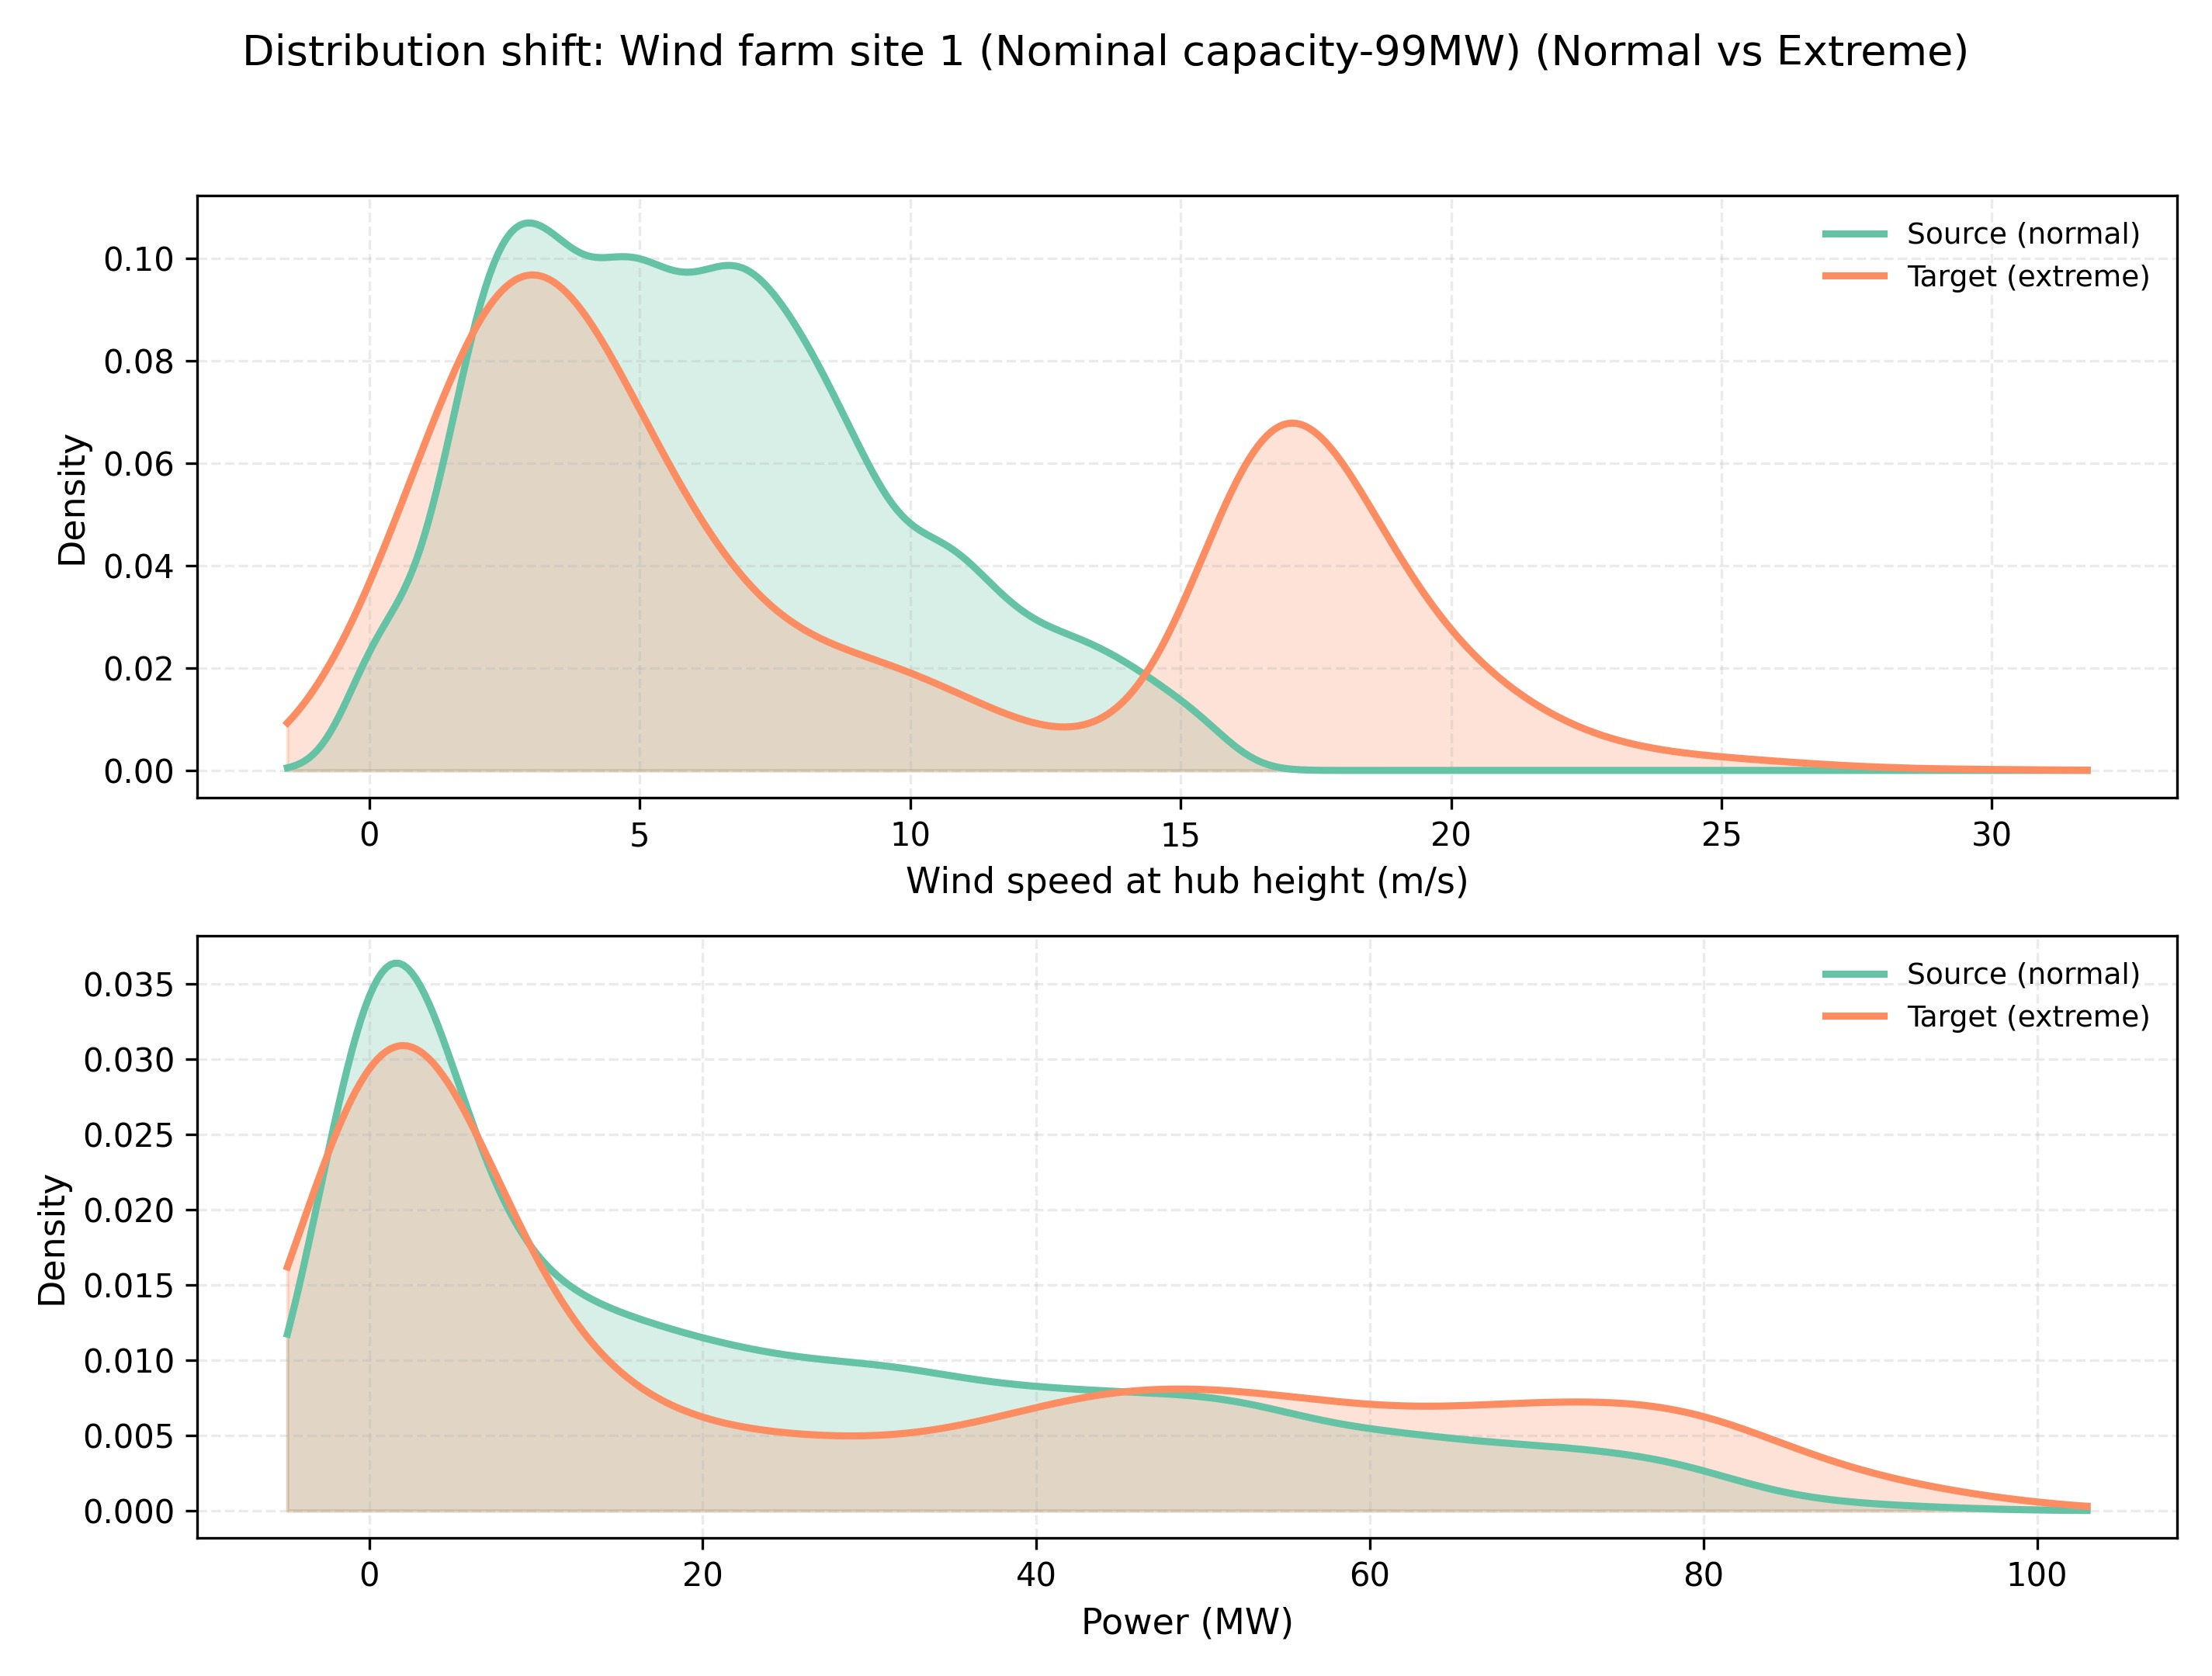
\includegraphics[width=0.46\textwidth]{experiment1/outputs/plots/farm1_domain_shift.jpg}
\hfill
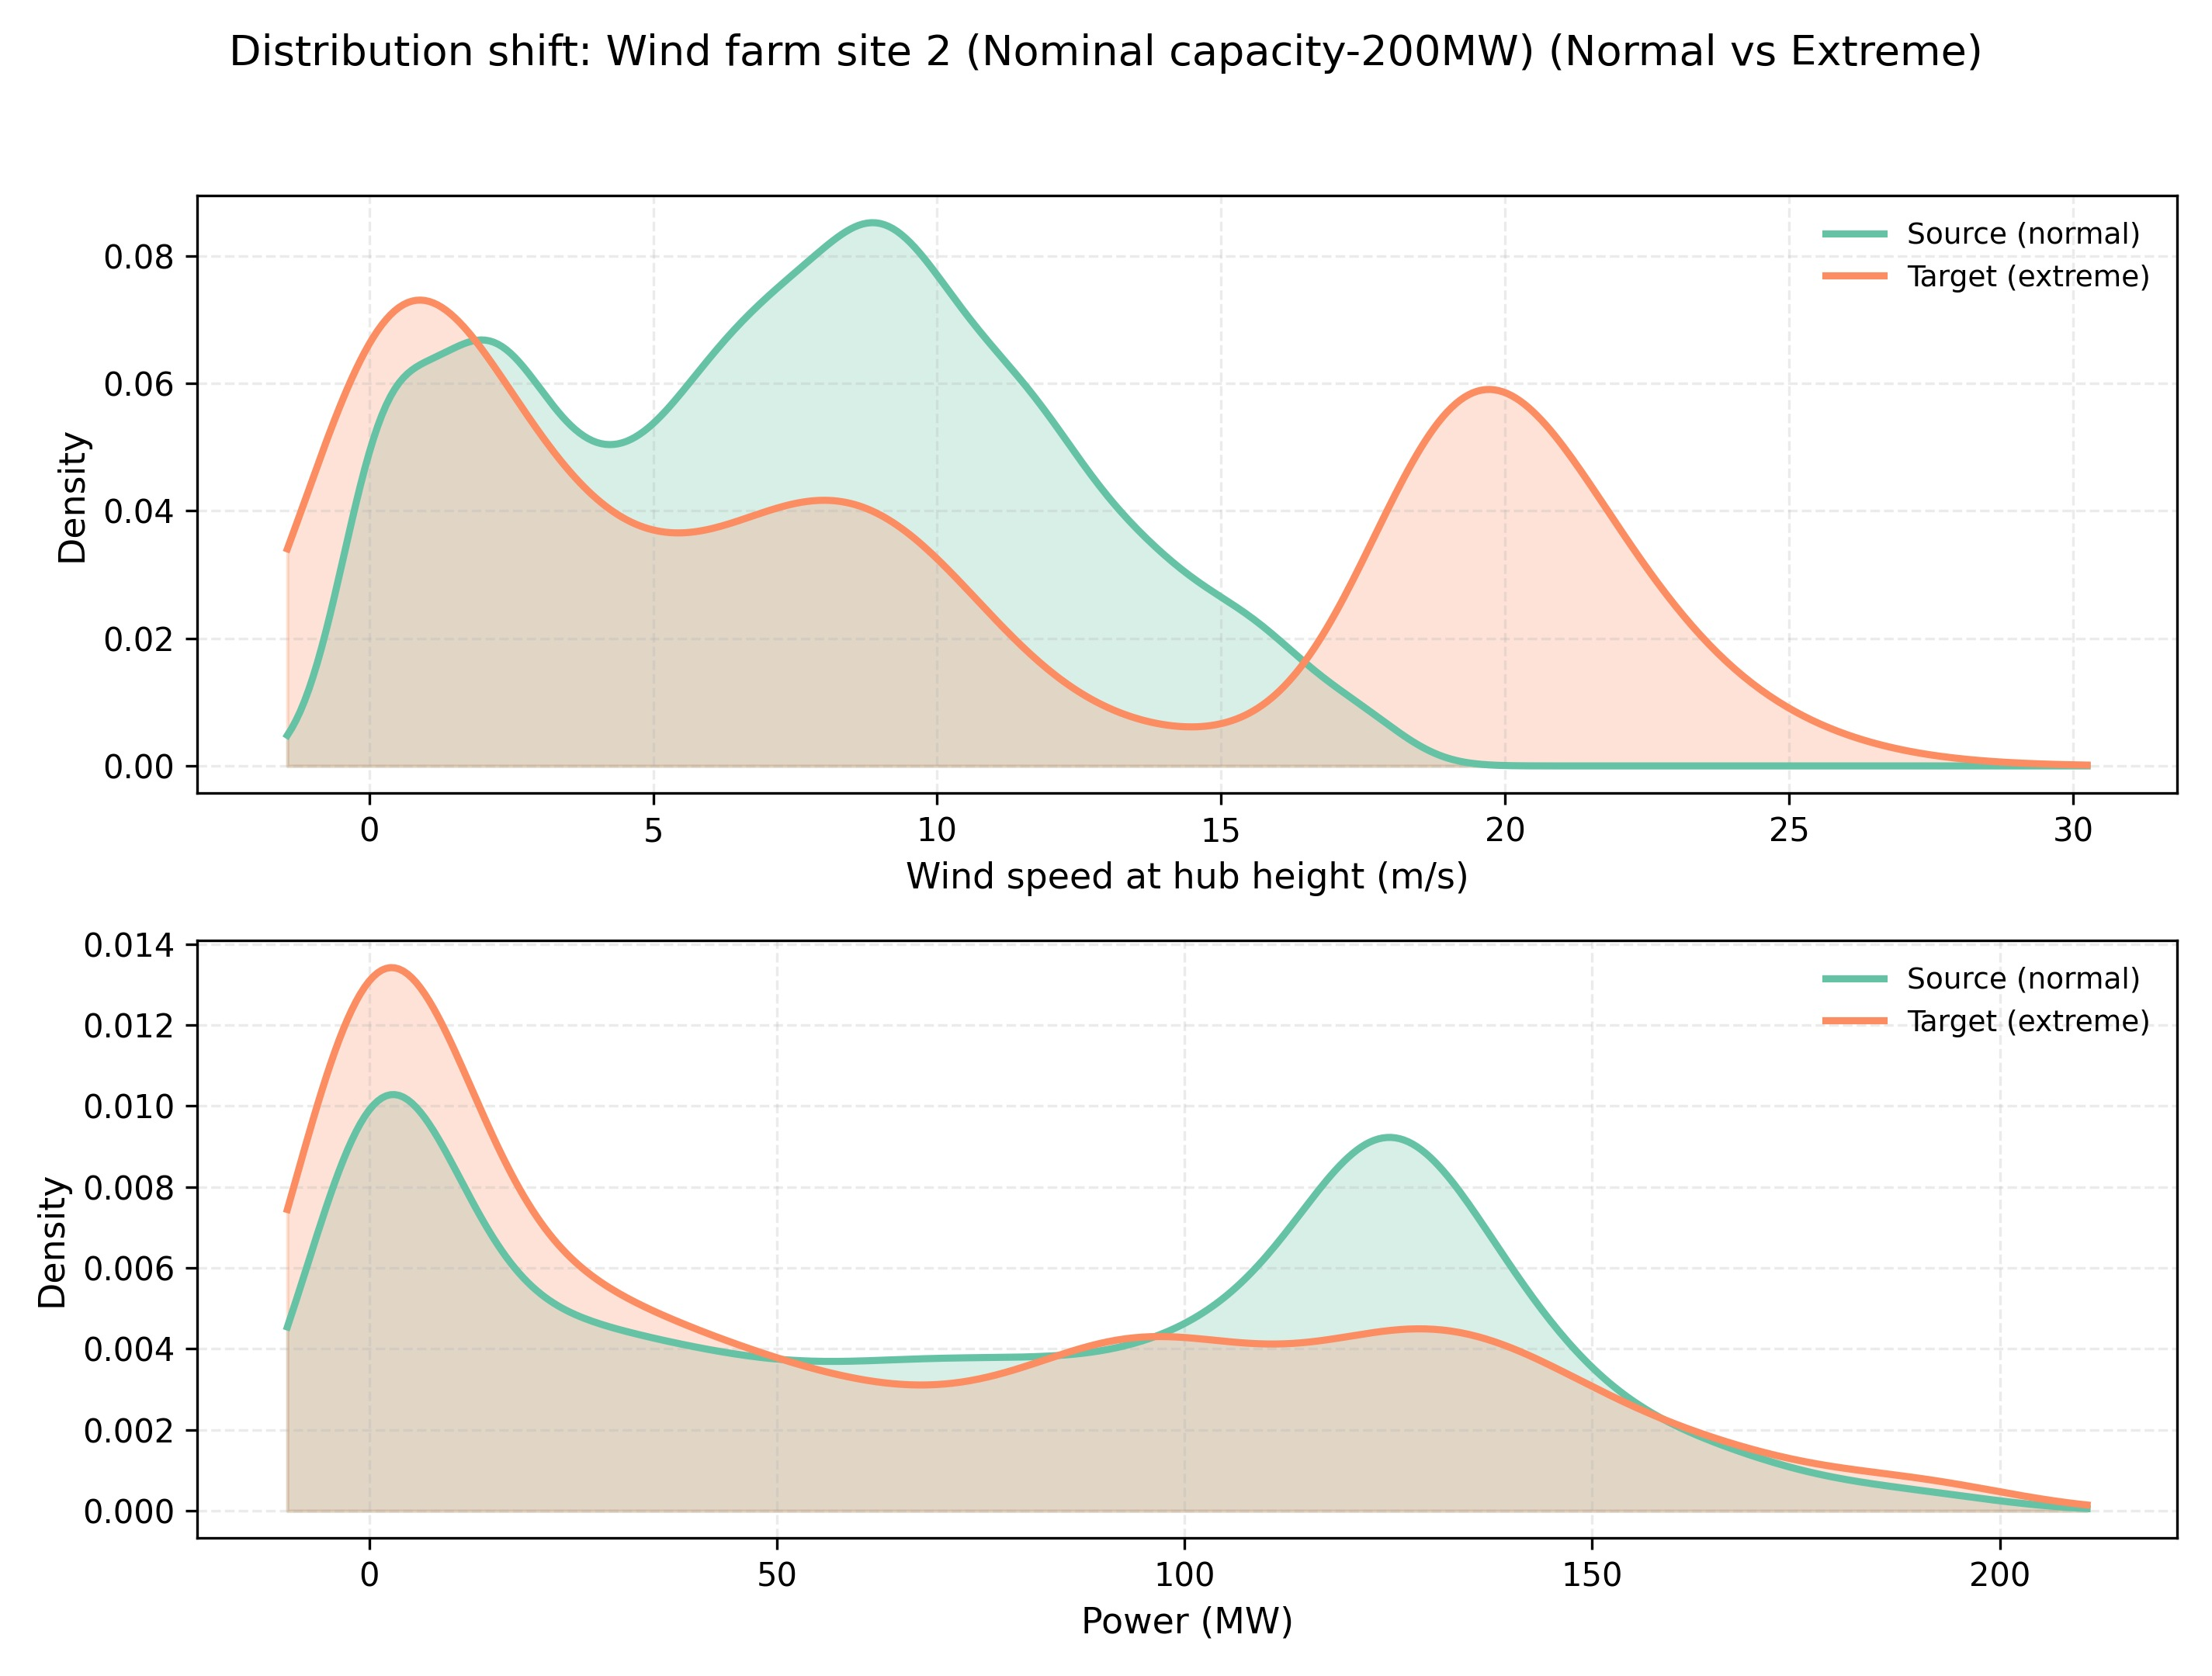
\includegraphics[width=0.46\textwidth]{experiment1/outputs/plots/farm0_domain_shift.jpg}

\vspace{0.12cm}
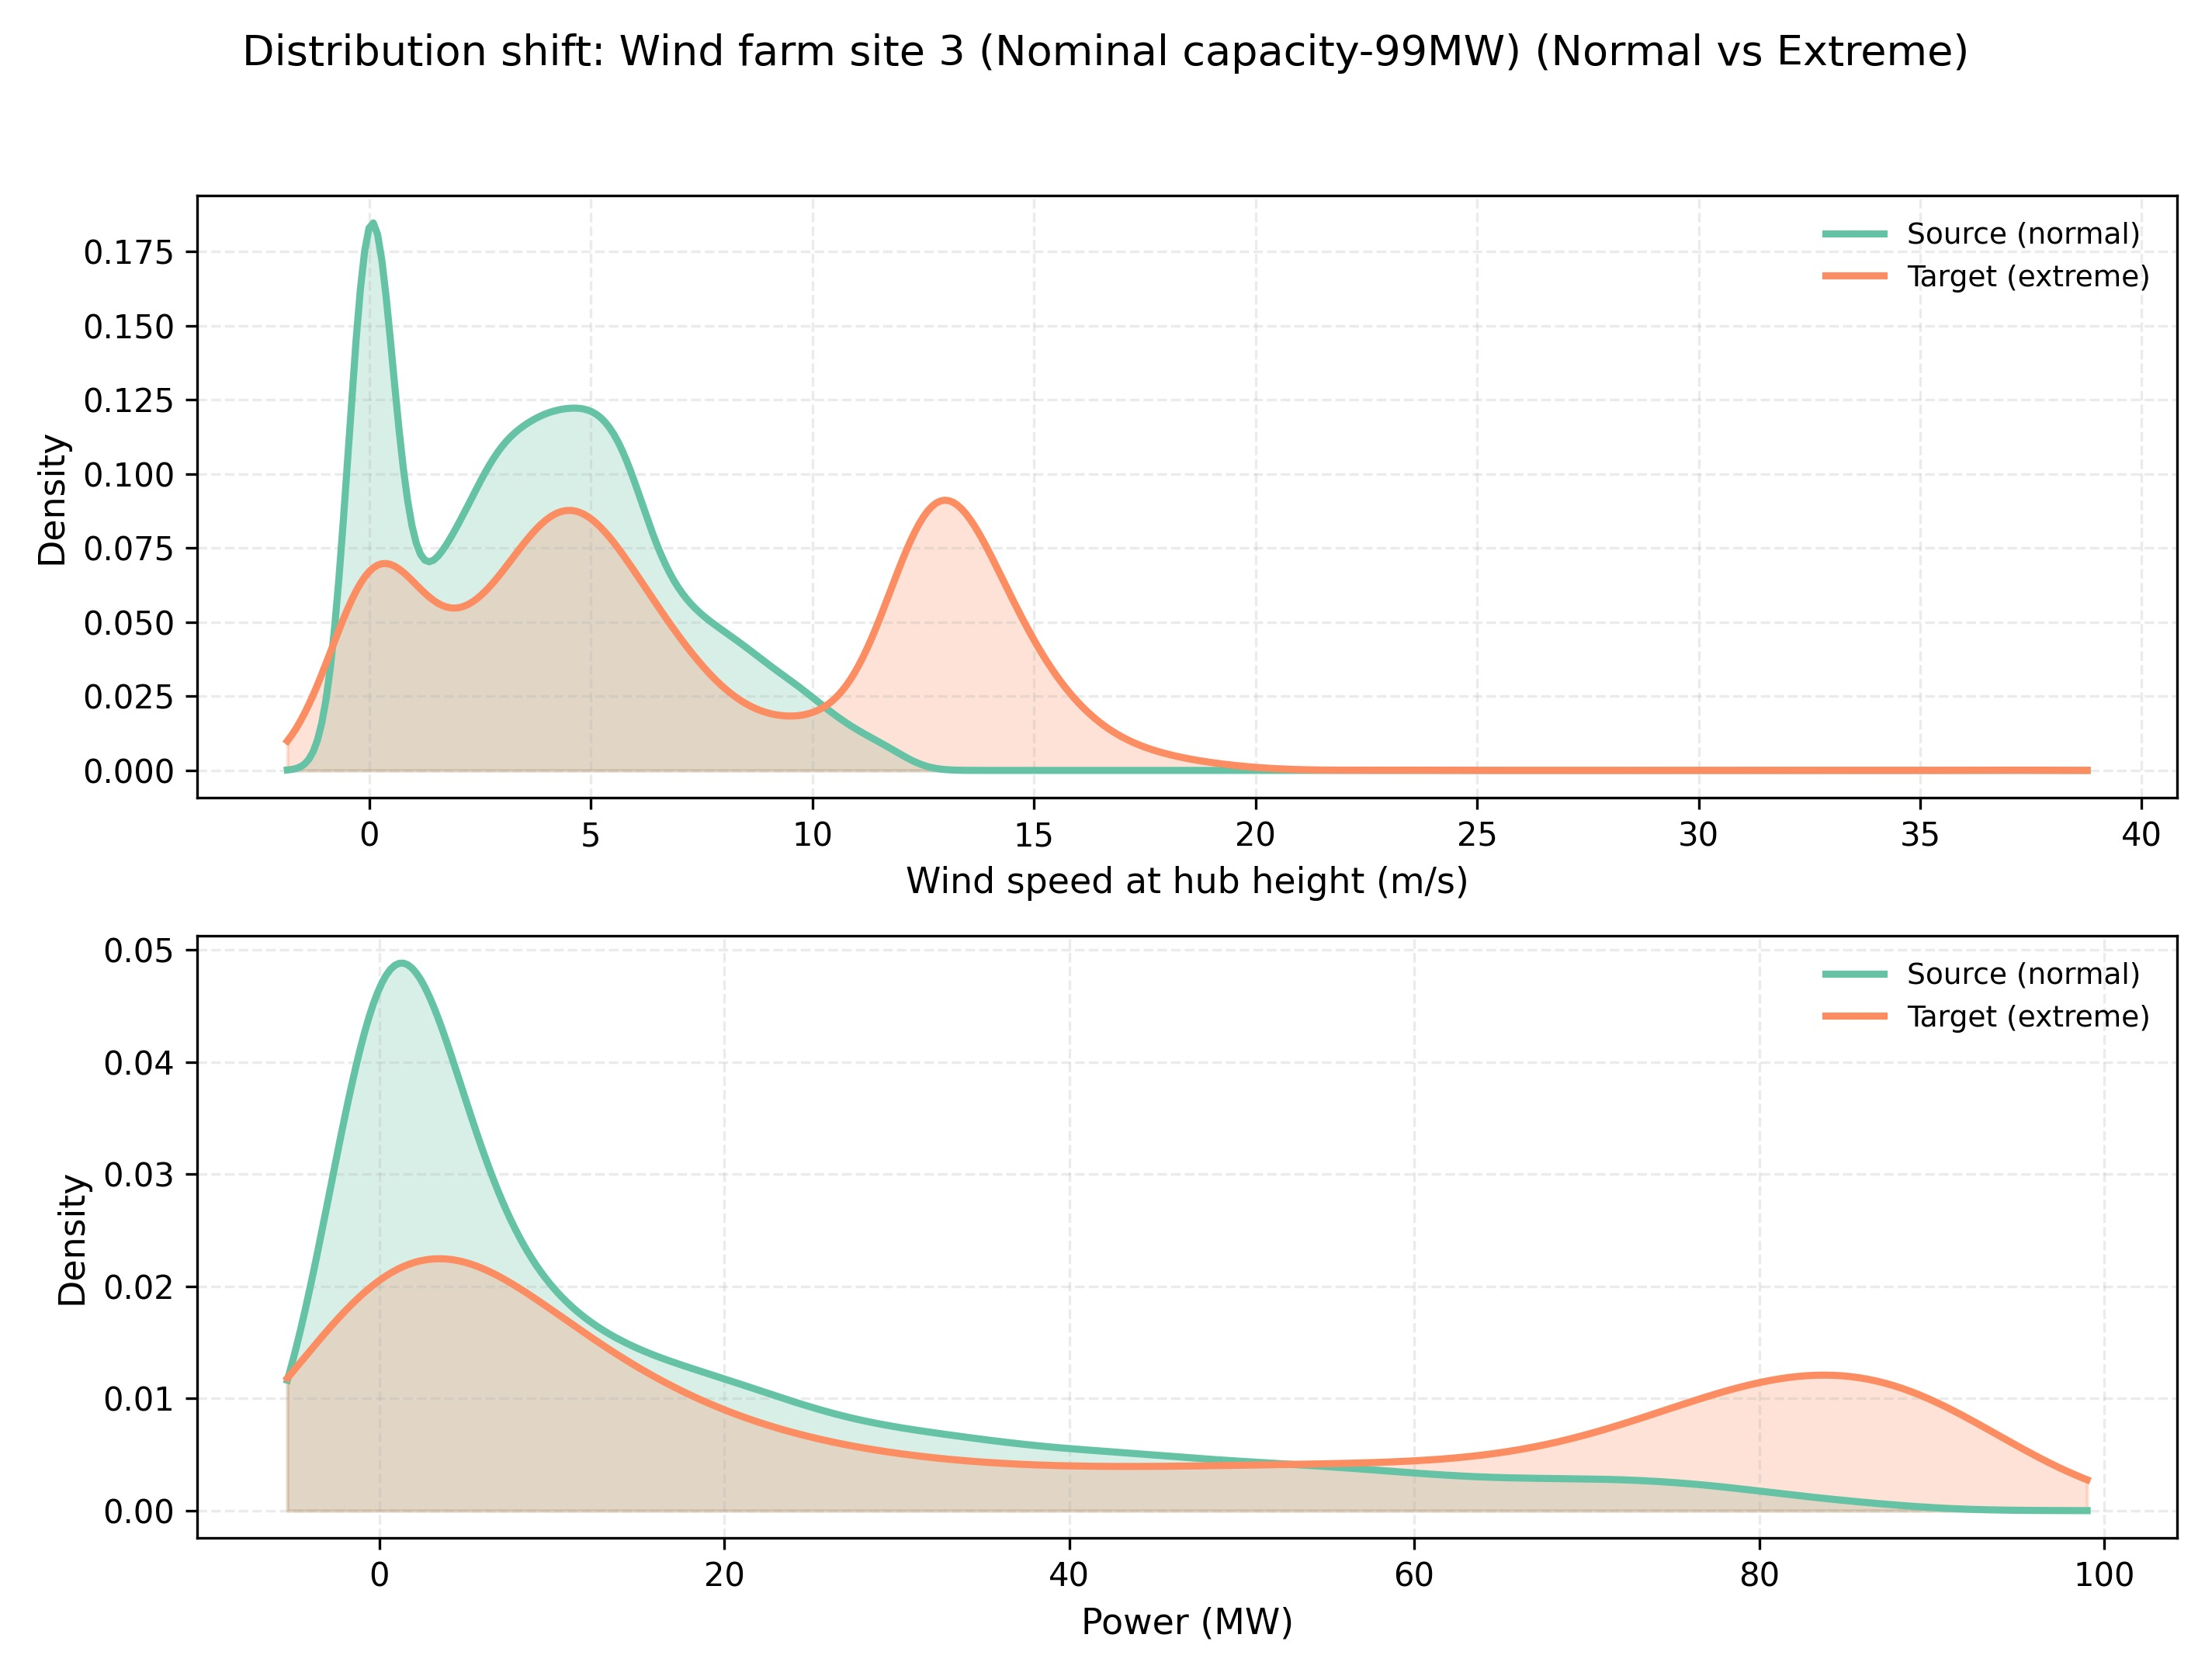
\includegraphics[width=0.46\textwidth]{experiment1/outputs/plots/farm2_domain_shift.jpg}
\hfill
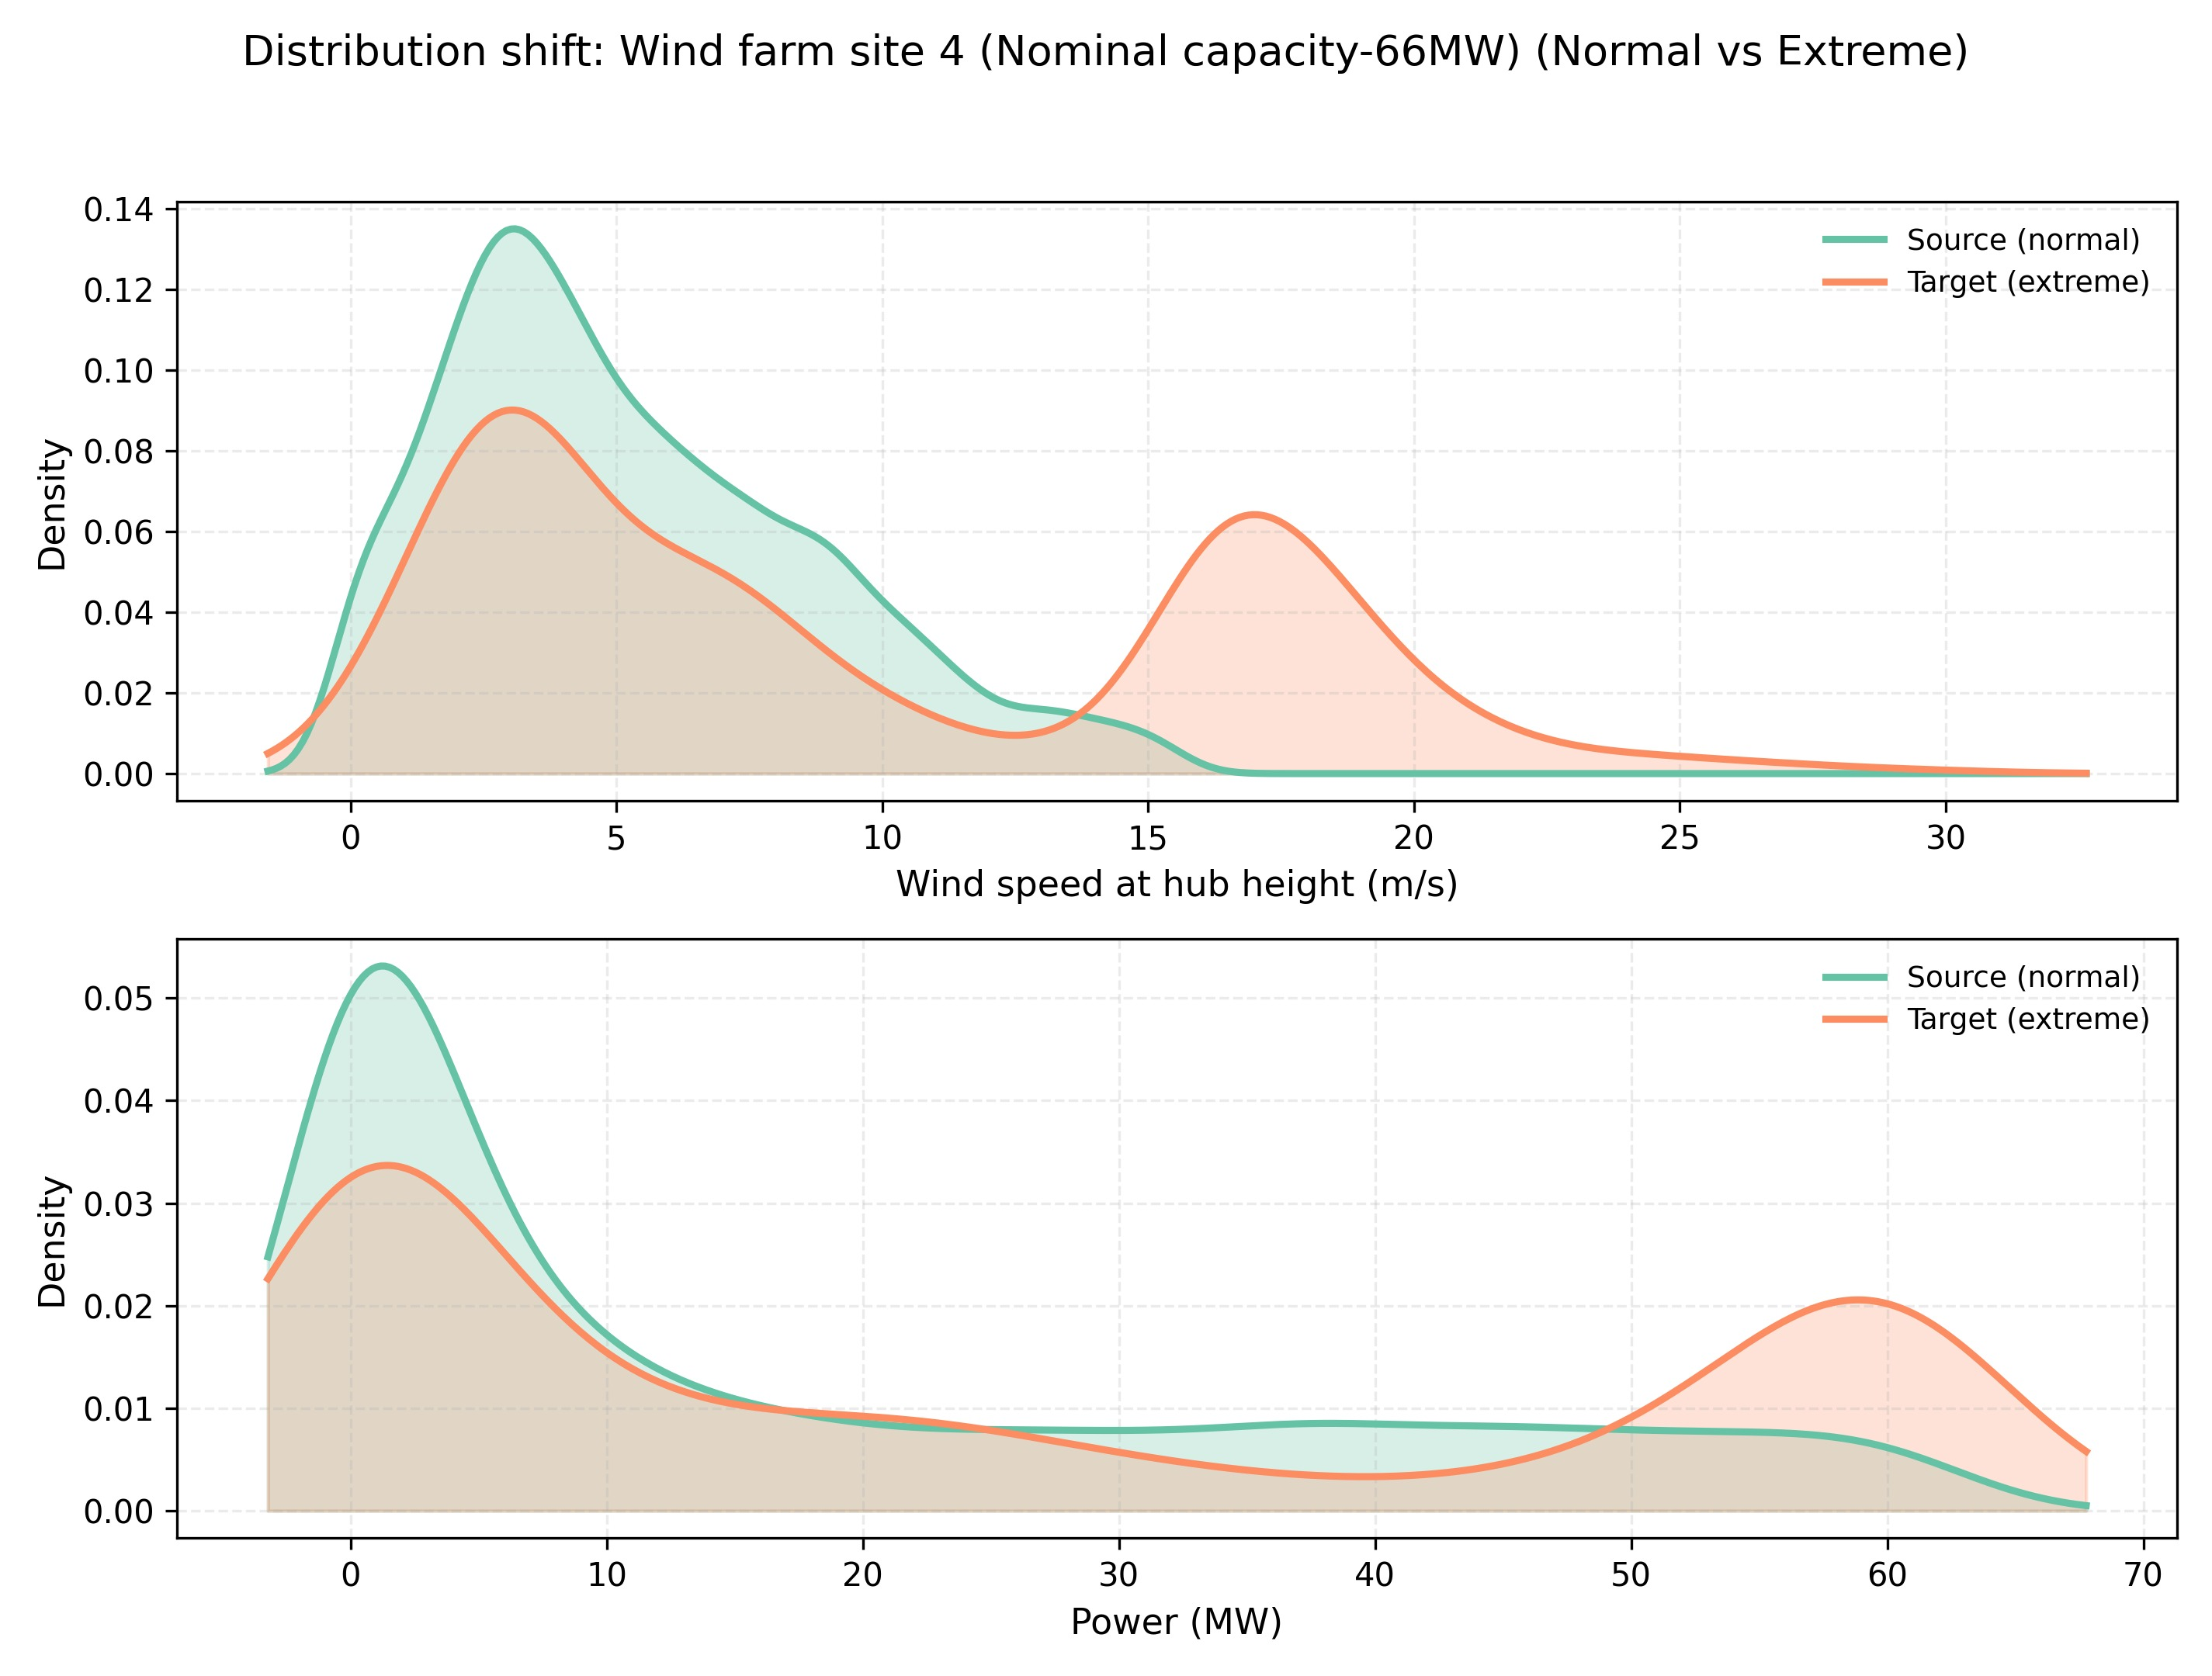
\includegraphics[width=0.46\textwidth]{experiment1/outputs/plots/farm4_domain_shift.jpg}

\vspace{0.12cm}
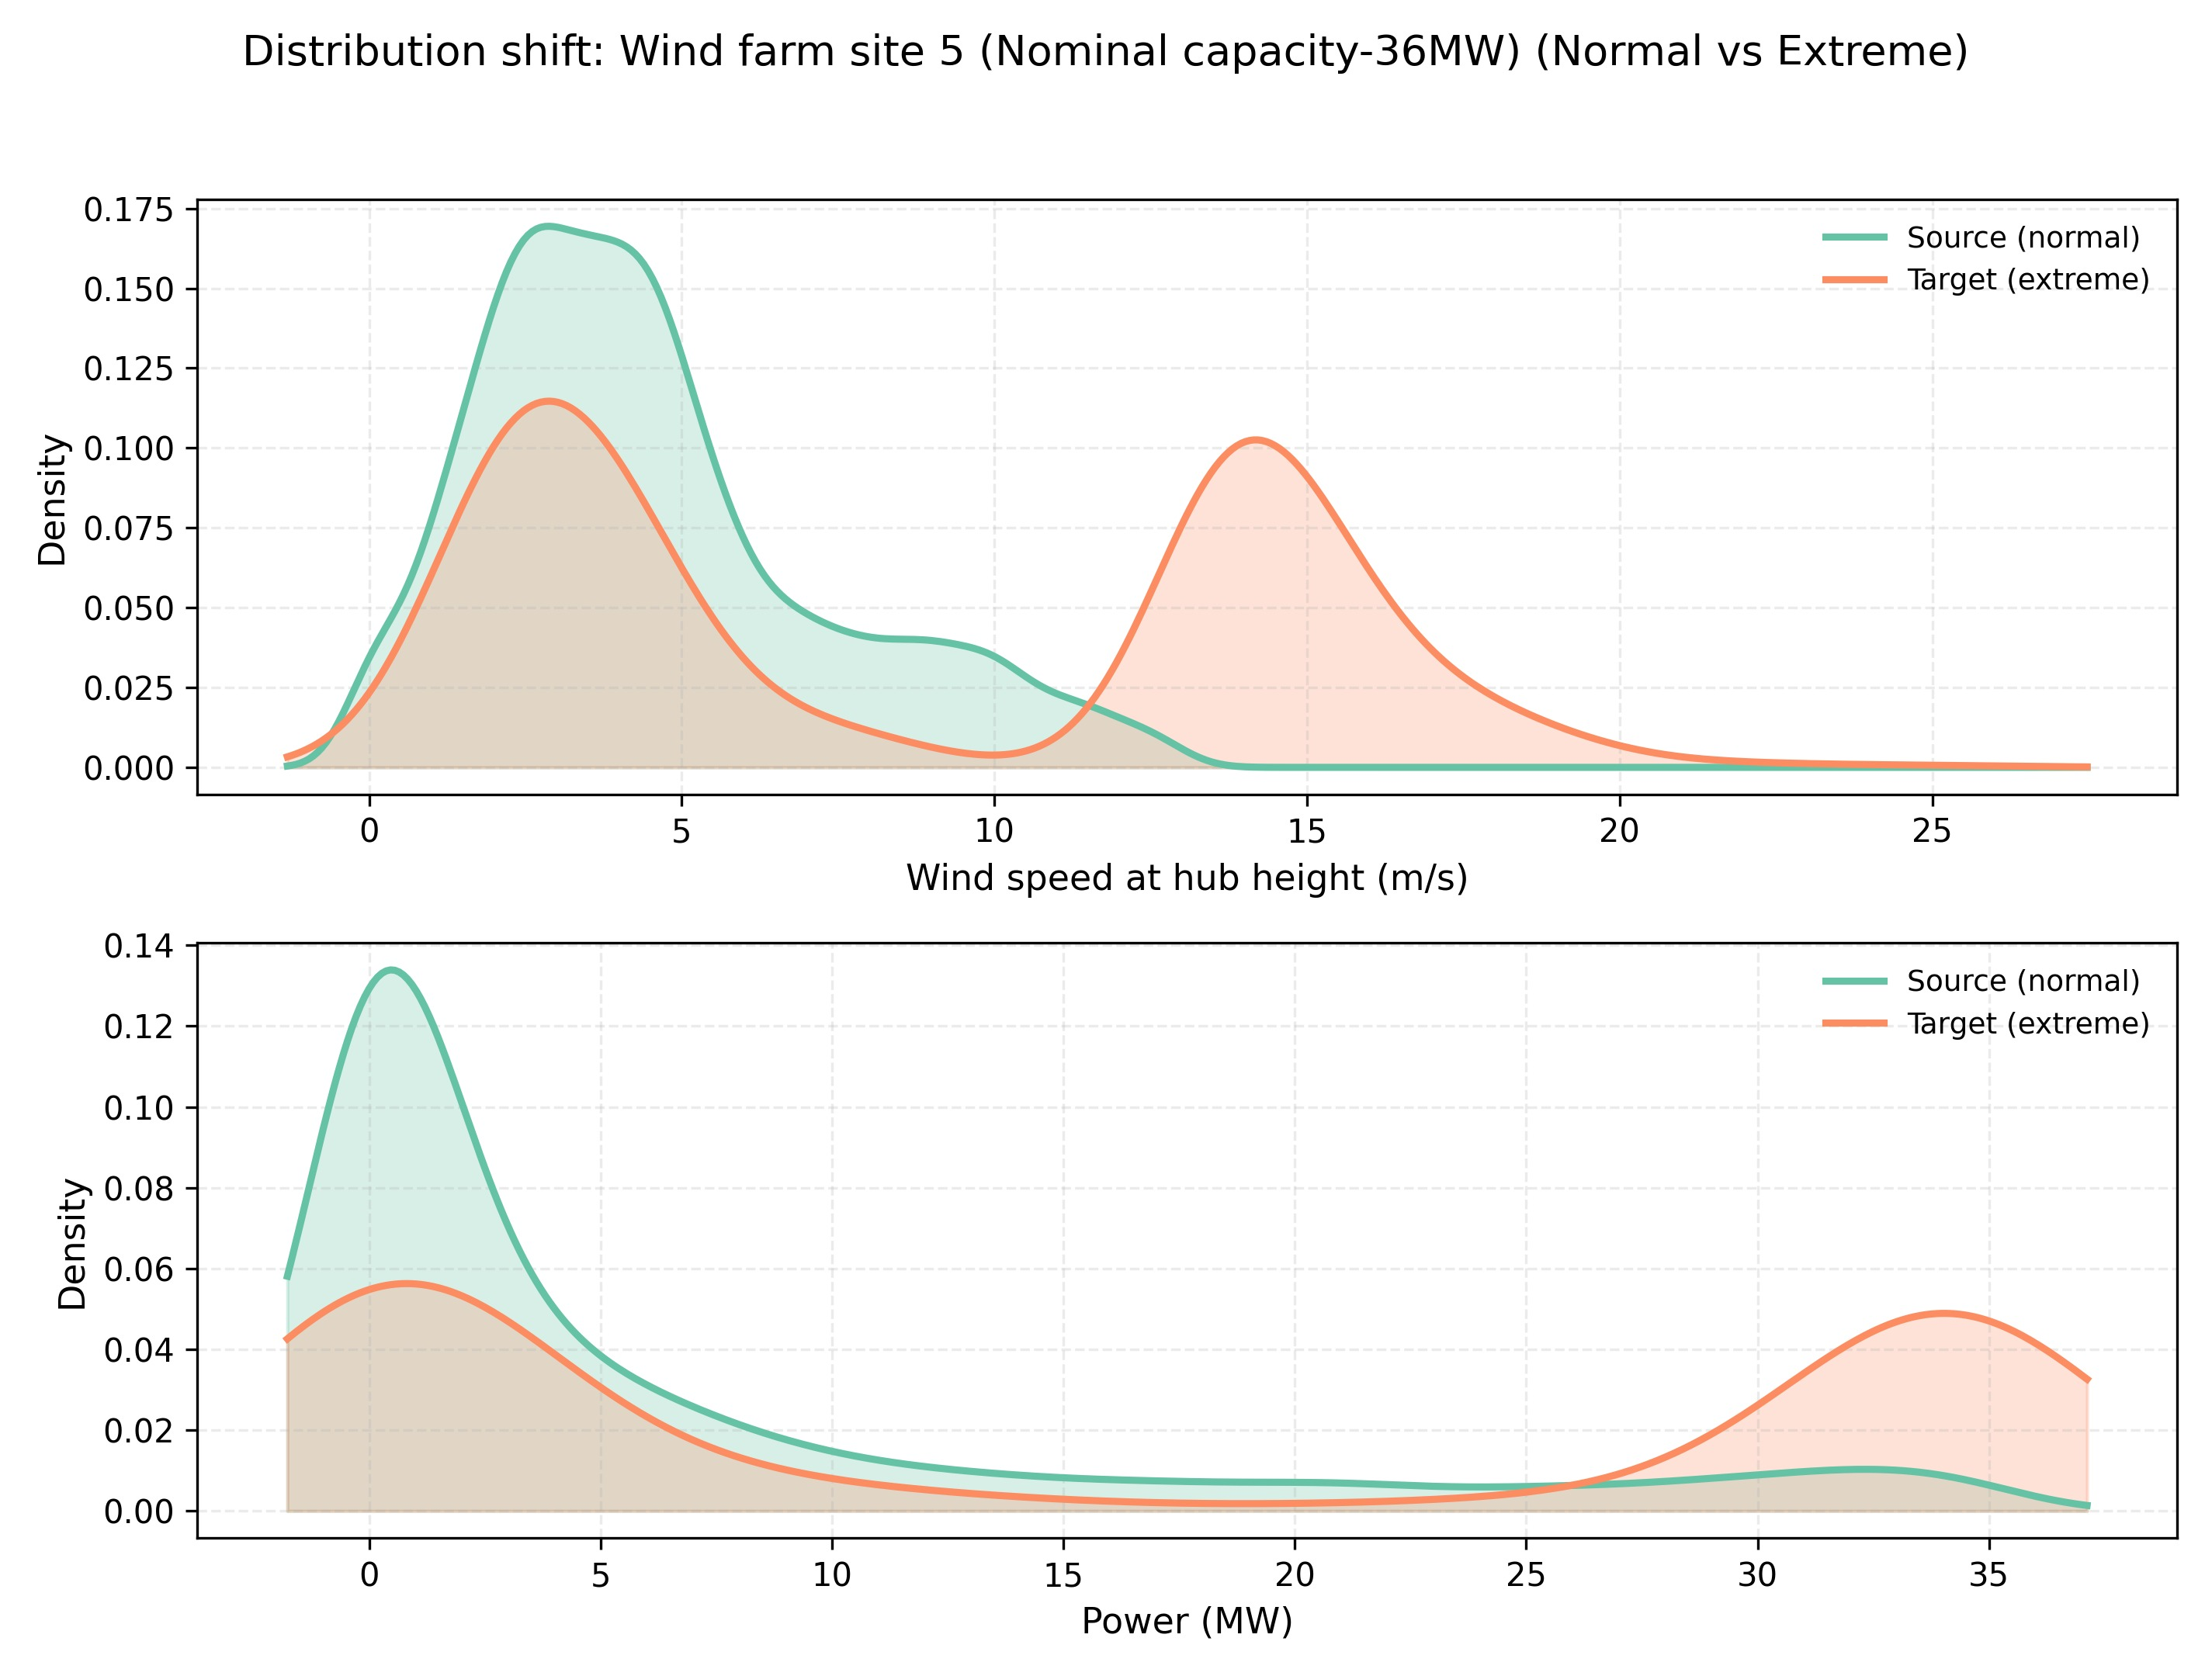
\includegraphics[width=0.46\textwidth]{experiment1/outputs/plots/farm5_domain_shift.jpg}
\hfill
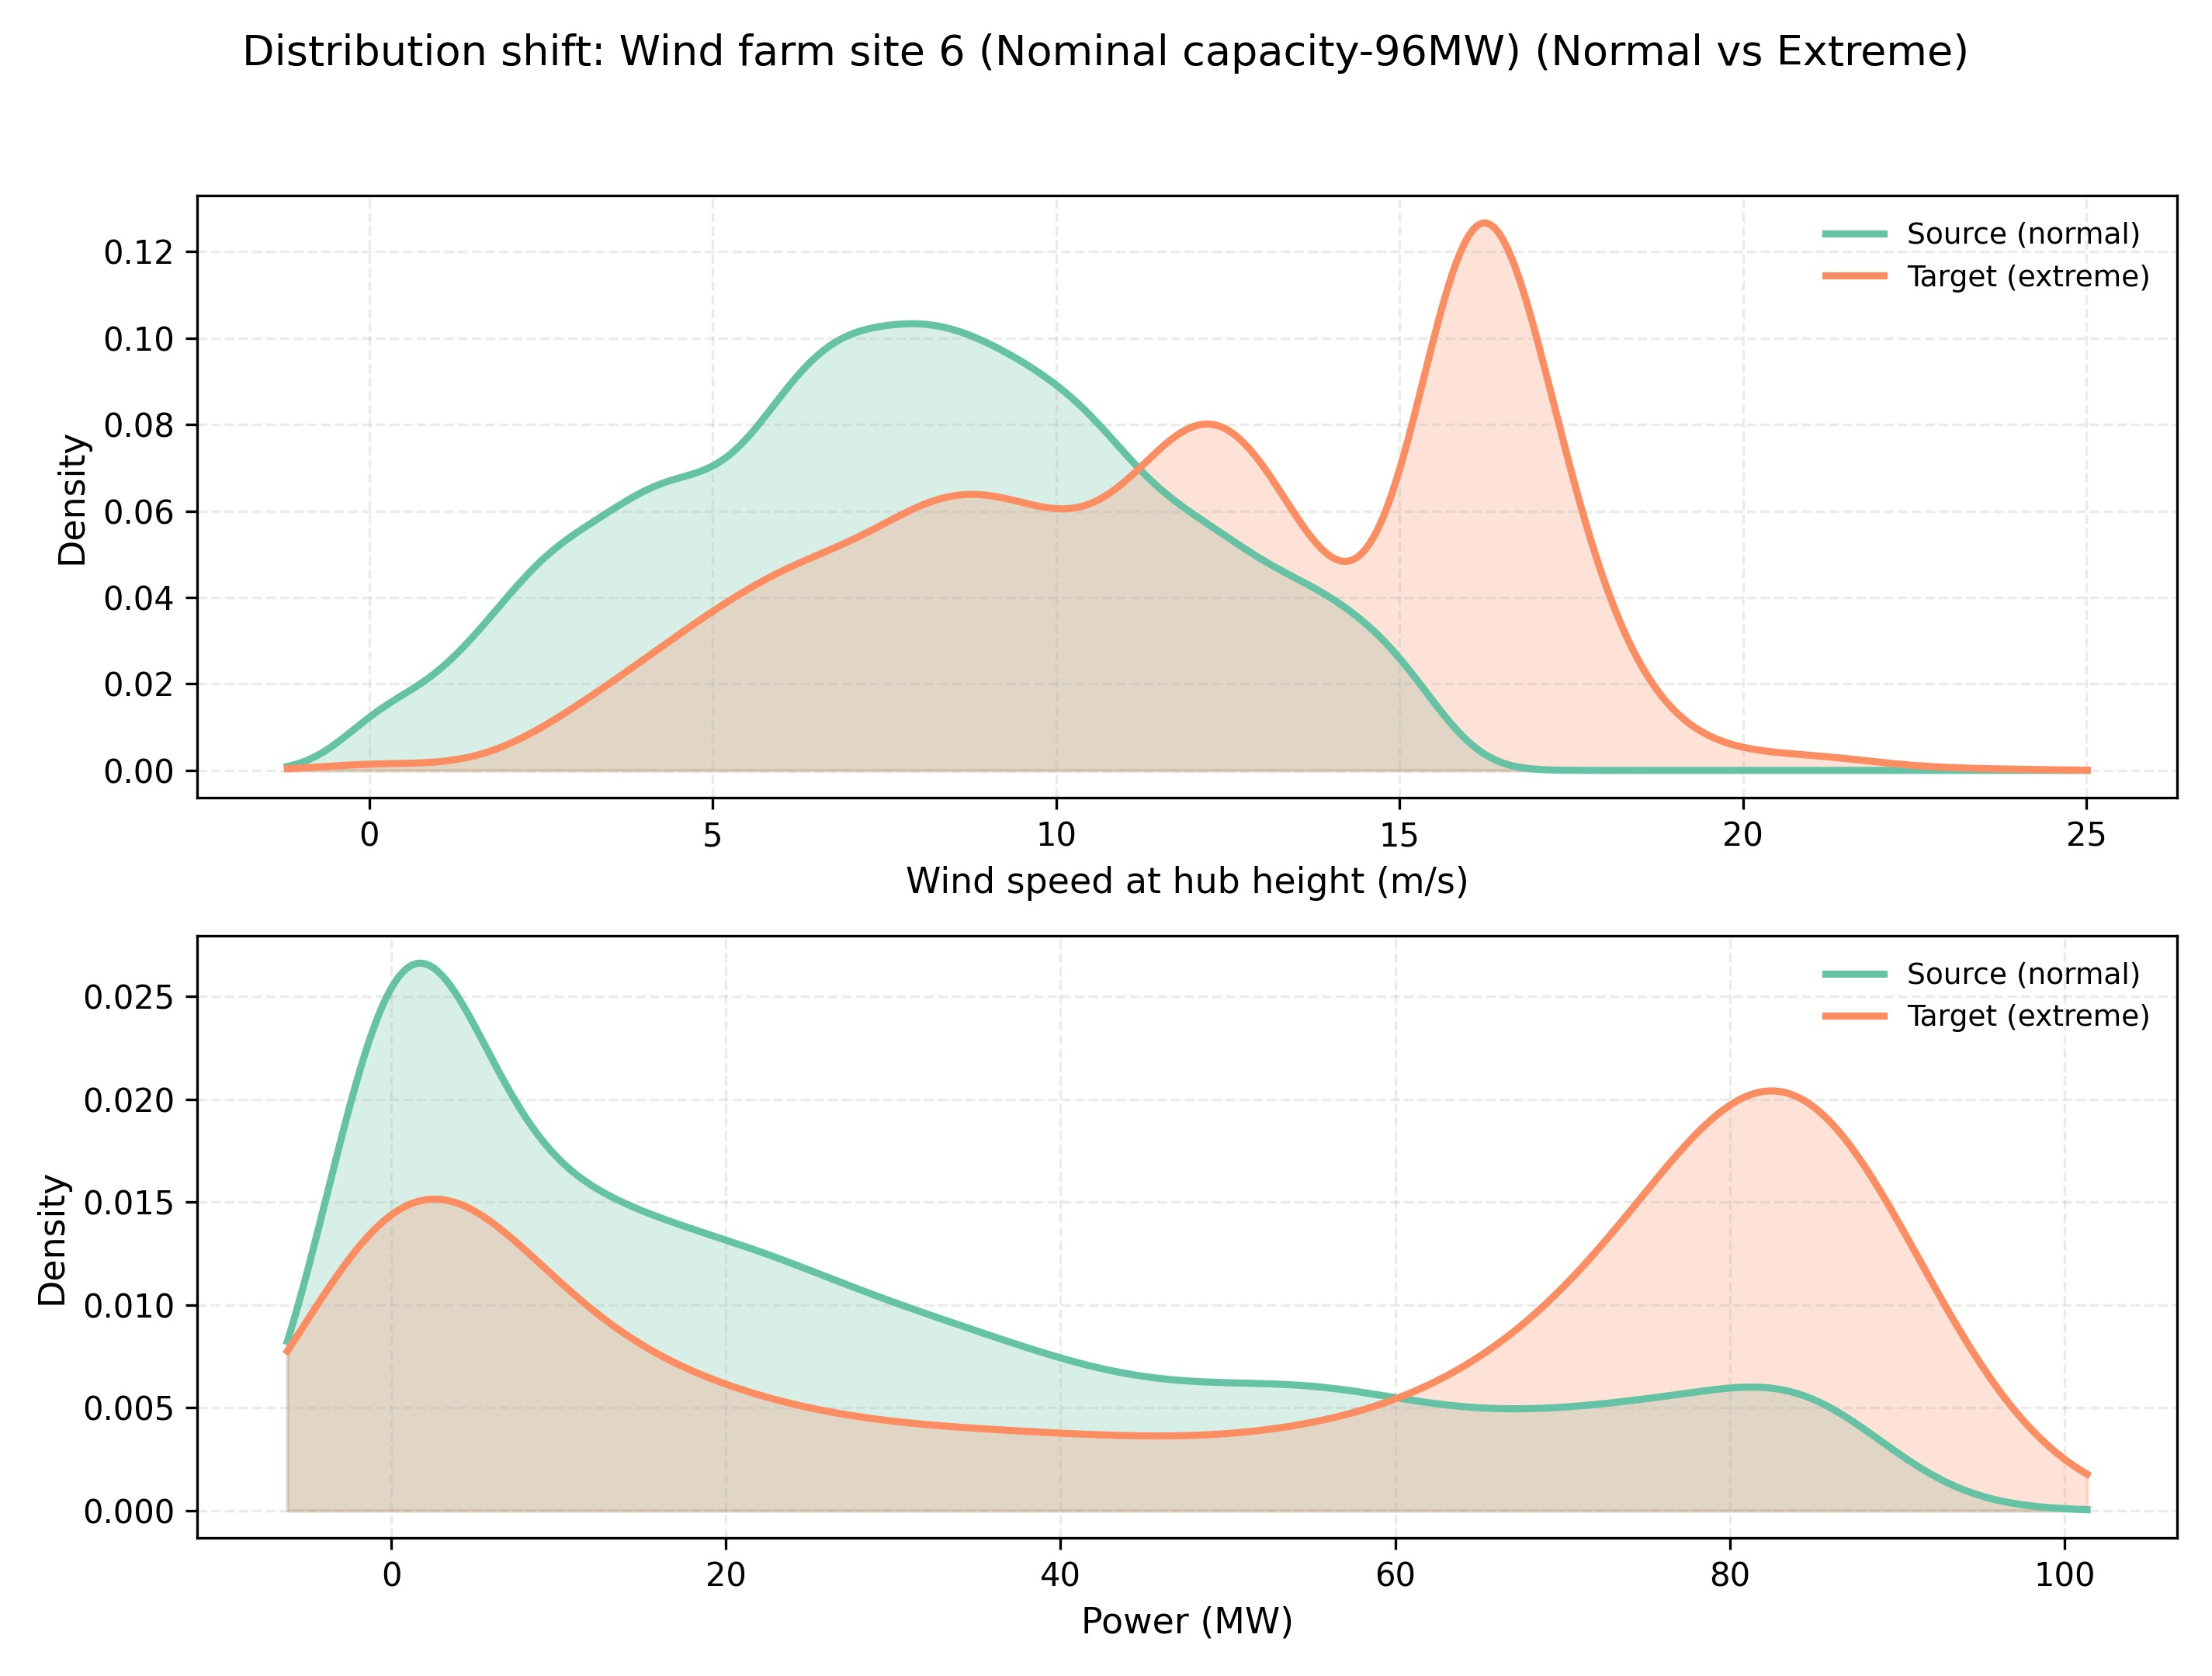
\includegraphics[width=0.46\textwidth]{experiment1/outputs/plots/farm3_domain_shift.jpg}
\caption{Distribution shift visualization for all six wind farms. From left to right, top to bottom: Site~1 (99\,MW), Site~2 (200\,MW), Site~3 (99\,MW), Site~4 (66\,MW), Site~5 (36\,MW), and Site~6 (96\,MW). Each subplot shows kernel density estimates of wind speed (upper panel) and power output (lower panel) for the normal-operating (source) and extreme-event (target) domains. {\color{blue}Site~6 has the largest power-domain Wasserstein distance in this historical comparison.}}
\label{fig:domain_shift}
\end{figure}

%---------------- Experiment 2 --------------------%
\subsection{Earlier point-prediction and noise experiments}\label{sec:exp2}

{\color{blue}The archived point-prediction comparison concerns Farm~6 and nine baselines under the original sample-splitting protocol. The model name in these tables and plots identifies the earlier implementation; its scores are not transferred to the corrected objective.}


The data partition for Farm~6 is as follows:
\begin{itemize}
    \item \textbf{Source domain} (normal operation): 66{,}009 samples;
    \item \textbf{Target domain} (extreme-event domain): 4{,}143 samples.
\end{itemize}

{\color{blue}The archived seed-0 random window split assigns 3,728 target samples to training and 415 to testing. These counts do not imply a chronological or event-separated holdout. The corrected-model diagnostic uses all 3,728 target-training labels for point prediction and separates 2,983 fitting labels from 745 calibration labels for intervals. All four variants are evaluated on the same 415 target test windows. The historical extreme-event thresholds were computed from full-record meteorological data, so they are not described as training-only estimates.}

We compare TL-QLDMR against nine baselines. The kernel-based baselines are SVR, LDMR, bounded-loss SVR (BLSSVR) \citep{fu2023bounded}, Harris hawks optimization SVR (HHO-SVR) \citep{houssein2025hho}, functional-iterative Lagrangian SVR (FLSVR) \citep{meena2025flsvr}, and associated-road-analysis SVR (ARA-SVR) \citep{duan2025ara}. The ensemble baselines are K-means clustering with gradient-boosted trees (KMeans-GBT) \citep{rizkallah2025kmeans}, random-forest wind power forecasting (RF-WPF) \citep{mustaffa2025rf}, and broad random-forest wind power forecasting (BRF-WPF) \citep{chen2025brf}.

\begin{table}[ht]
\centering
\caption{{\color{blue}Archived manuscript values (not recomputed): }Deterministic point prediction results on the extreme-event test set of Farm~6. Best results are highlighted in bold (similarly hereinafter).}
\setlength{\tabcolsep}{3.5mm}
\begin{tabular}{lccc}
\toprule
Model & RMSE & MAE & $R^2$ \\
\midrule
LDMR & 10.692 & 6.327 & 0.9085 \\
BLSSVR        & 10.273 & 6.140 & 0.9155 \\
ARA-SVR       & 9.246 & 5.954 & 0.9316 \\
FLSVR         & 8.794 & 6.301 & 0.9381 \\
SVR  & 8.564 & 5.537 & 0.9413 \\
HHO-SVR       & 7.603 & 5.530 & 0.9537 \\
BRF-WPF       & 9.719 & 6.870 & 0.9244 \\
KMeans-GBT    & 9.620 & 6.695 & 0.9259 \\
RF-WPF        & 7.967 & 5.344 & 0.9492 \\
\textbf{TL-QLDMR (Ours)} & \textbf{7.478} & \textbf{5.248} & \textbf{0.9557} \\
\bottomrule
\end{tabular}
\label{tab:exp2_results}
\end{table}

\begin{figure}
\centering
\begin{minipage}[t]{0.49\linewidth}
\centering
(a) LDMR\par
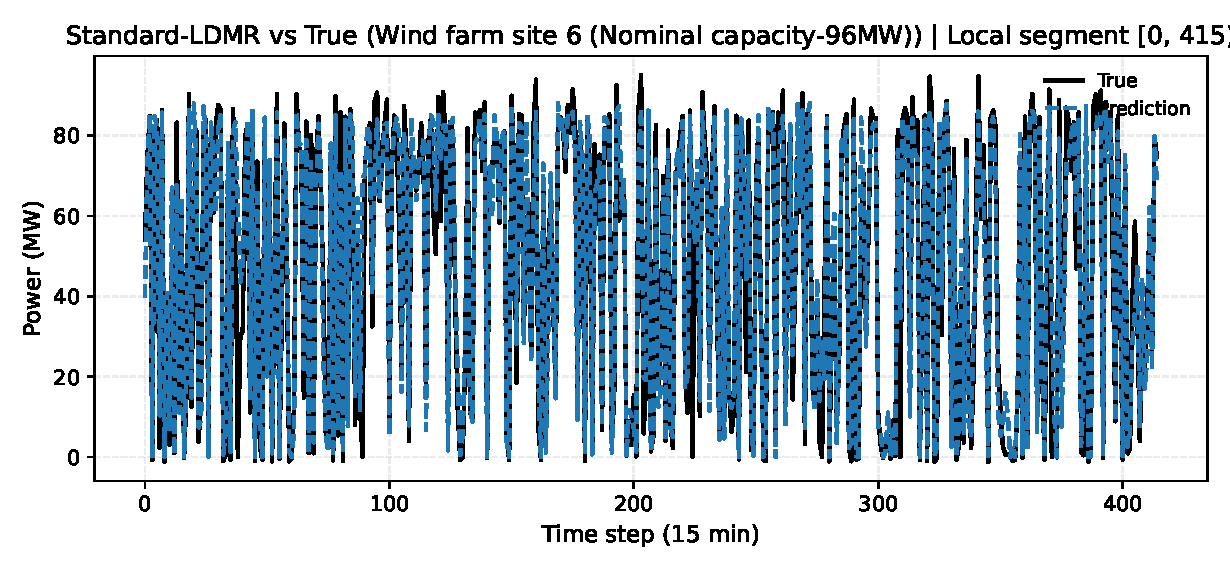
\includegraphics[width=\linewidth]{experiment2/plots_selected/farm3_Standard-LDMR.pdf}
\end{minipage}\hfill
\begin{minipage}[t]{0.49\linewidth}
\centering
(b) BLSSVR\par
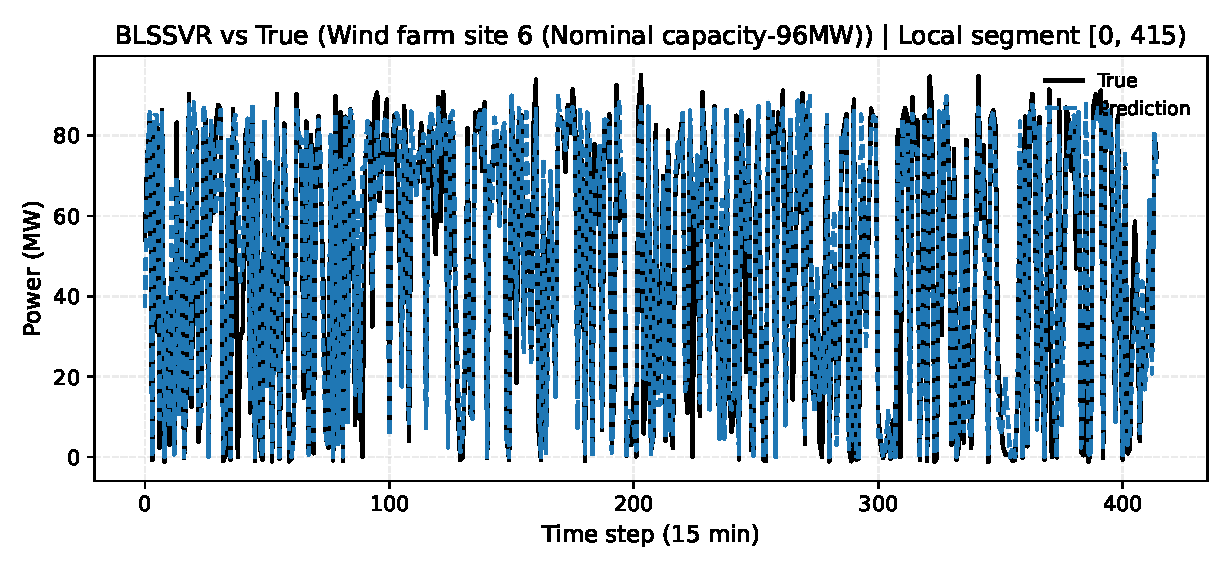
\includegraphics[width=\linewidth]{experiment2/plots_selected/farm3_BLSSVR.pdf}
\end{minipage}
\caption{{\color{blue}Archived manuscript values (not recomputed): }Prediction comparison over selected temporal segments on the Farm~6 extreme-event test set (Part I).}
\label{fig:exp2_curves_a}
\end{figure}

\begin{figure}
\centering
\begin{minipage}[t]{0.49\linewidth}
\centering
(c) ARA-SVR\par
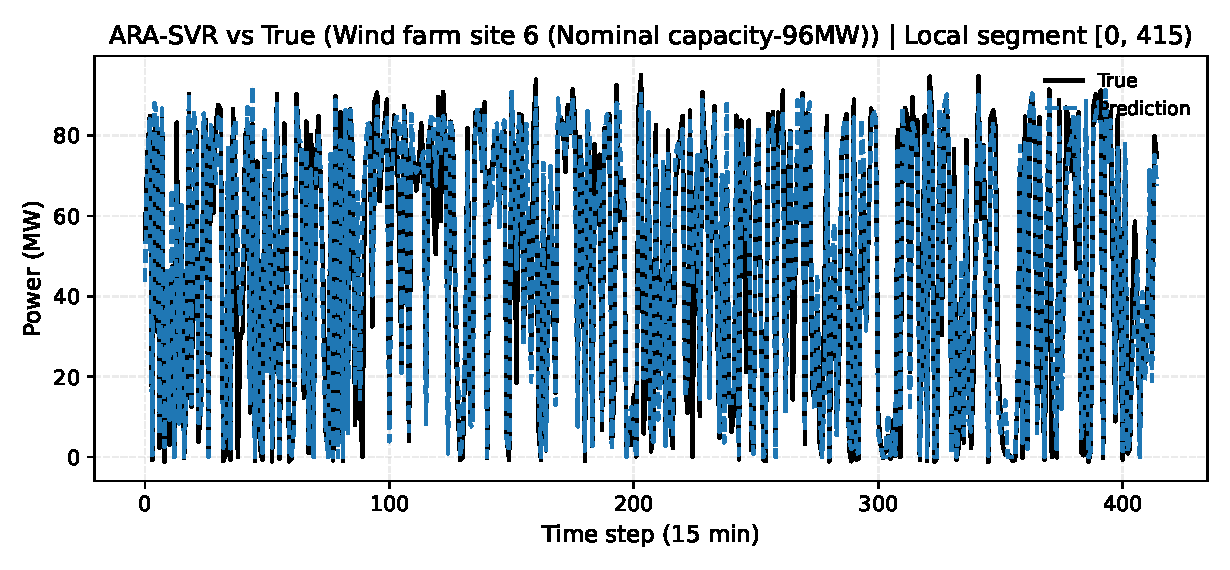
\includegraphics[width=\linewidth]{experiment2/plots_selected/farm3_ARA-SVR.pdf}
\end{minipage}\hfill
\begin{minipage}[t]{0.49\linewidth}
\centering
(d) FLSVR\par
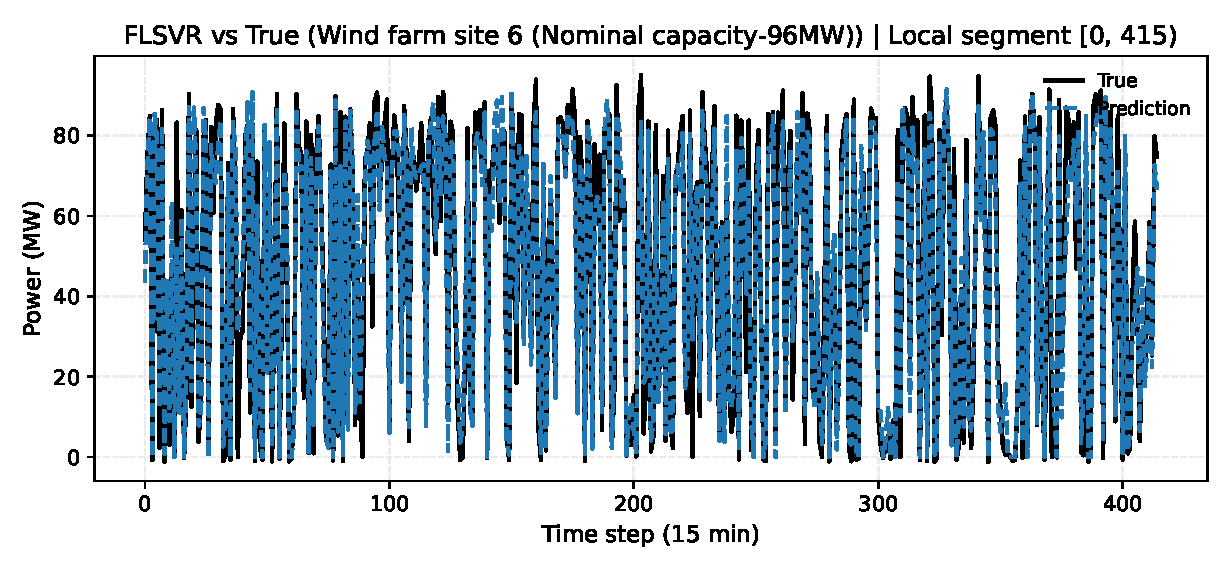
\includegraphics[width=\linewidth]{experiment2/plots_selected/farm3_FLSVR.pdf}
\end{minipage}
\caption{{\color{blue}Archived manuscript values (not recomputed): }Prediction comparison over selected temporal segments on the Farm~6 extreme-event test set (Part II).}
\label{fig:exp2_curves_b}
\end{figure}

\begin{figure}
\centering
\begin{minipage}[t]{0.49\linewidth}
\centering
(e) SVR\par
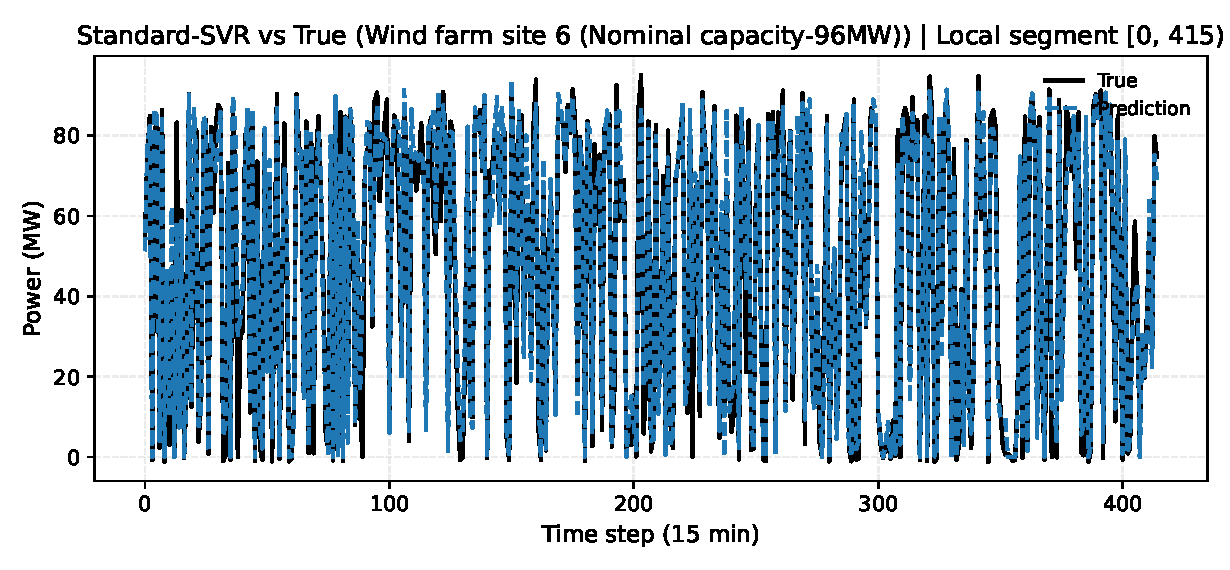
\includegraphics[width=\linewidth]{experiment2/plots_selected/farm3_Standard-SVR.pdf}
\end{minipage}\hfill
\begin{minipage}[t]{0.49\linewidth}
\centering
(f) HHO-SVR\par
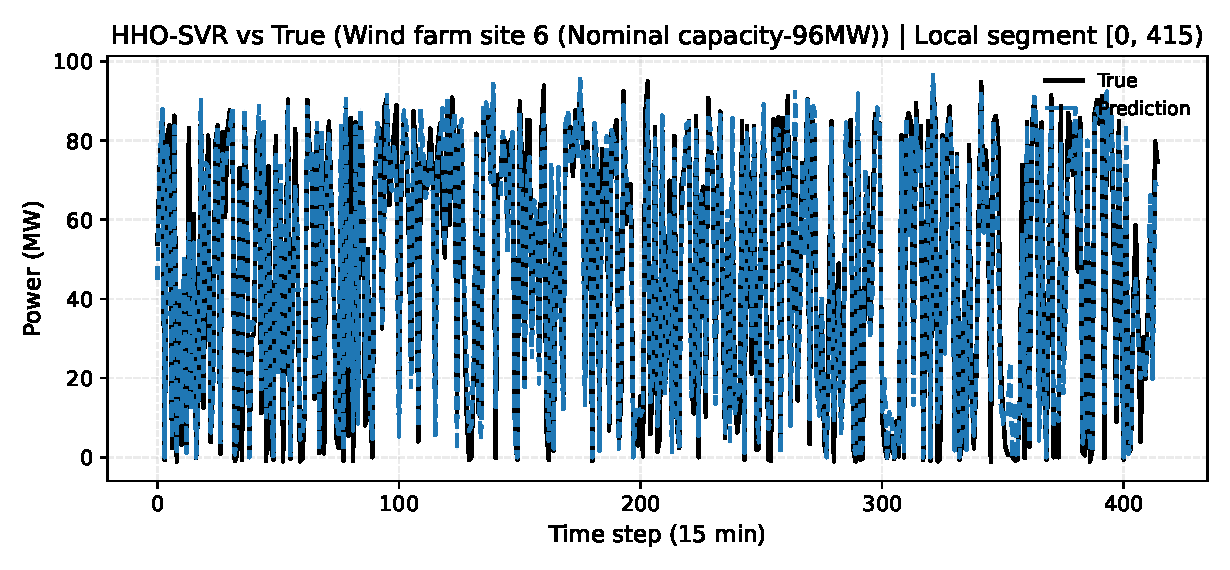
\includegraphics[width=\linewidth]{experiment2/plots_selected/farm3_HHO-SVR.pdf}
\end{minipage}
\caption{{\color{blue}Archived manuscript values (not recomputed): }Prediction comparison over selected temporal segments on the Farm~6 extreme-event test set (Part III).}
\label{fig:exp2_curves_c}
\end{figure}

\begin{figure}
\centering
\begin{minipage}[t]{0.49\linewidth}
\centering
(g) BRF-WPF\par
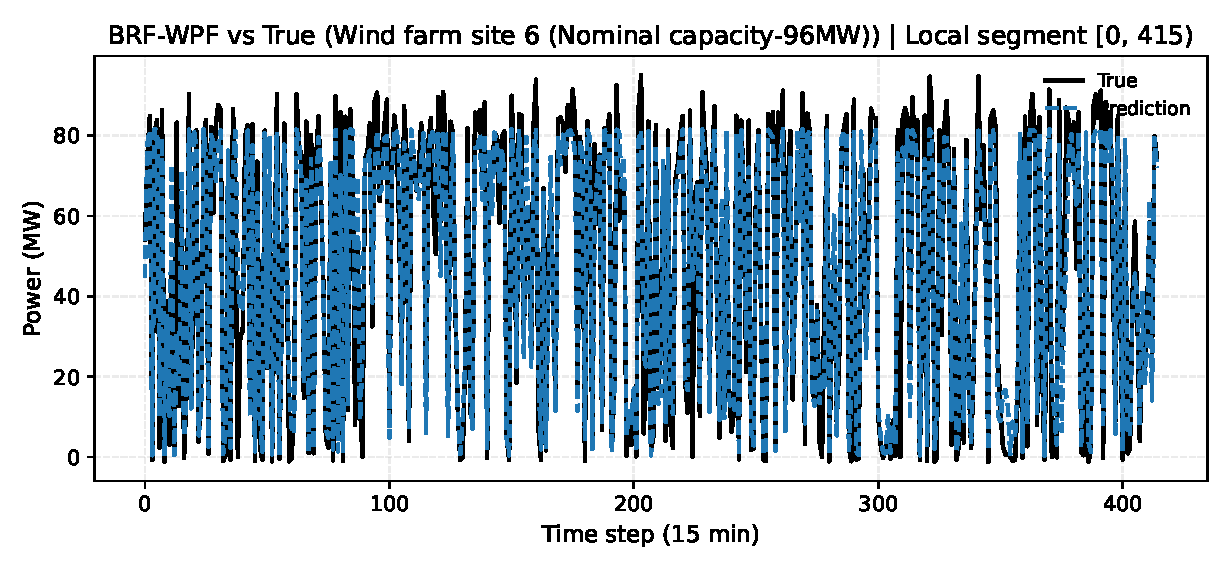
\includegraphics[width=\linewidth]{experiment2/plots_selected/farm3_BRF-WPF.pdf}
\end{minipage}\hfill
\begin{minipage}[t]{0.49\linewidth}
\centering
(h) KMeans-GBT\par
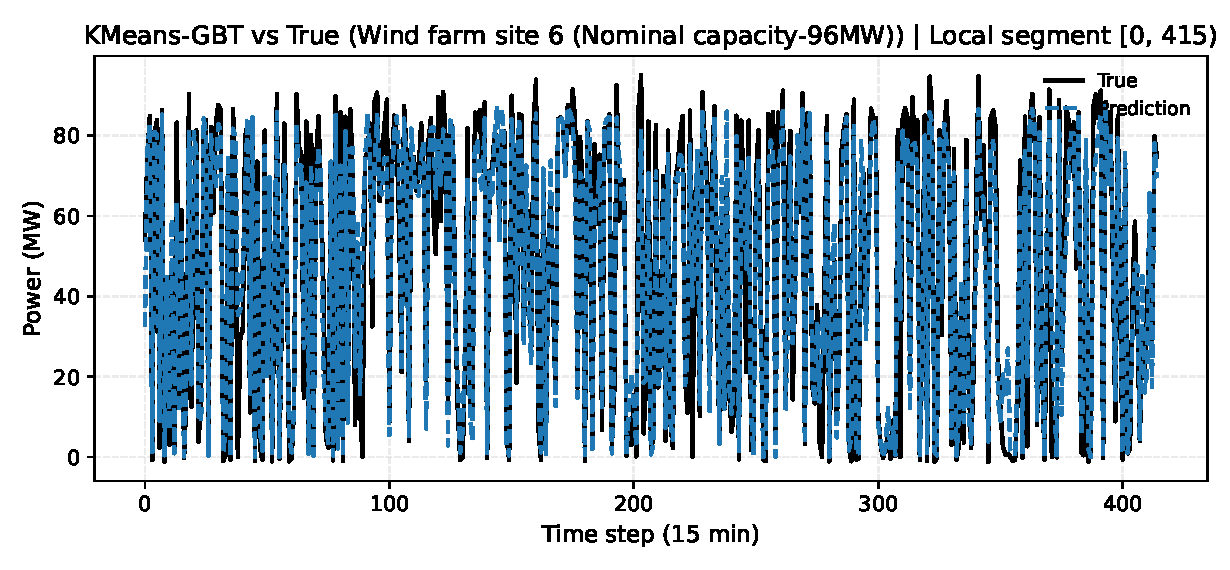
\includegraphics[width=\linewidth]{experiment2/plots_selected/farm3_KMeans-GBT.pdf}
\end{minipage}
\caption{{\color{blue}Archived manuscript values (not recomputed): }Prediction comparison over selected temporal segments on the Farm~6 extreme-event test set (Part IV).}
\label{fig:exp2_curves_d}
\end{figure}

\begin{figure}[htbp]
\centering
\captionsetup{type=figure}
\begin{minipage}[t]{0.47\linewidth}
\centering
(i) RF-WPF\par
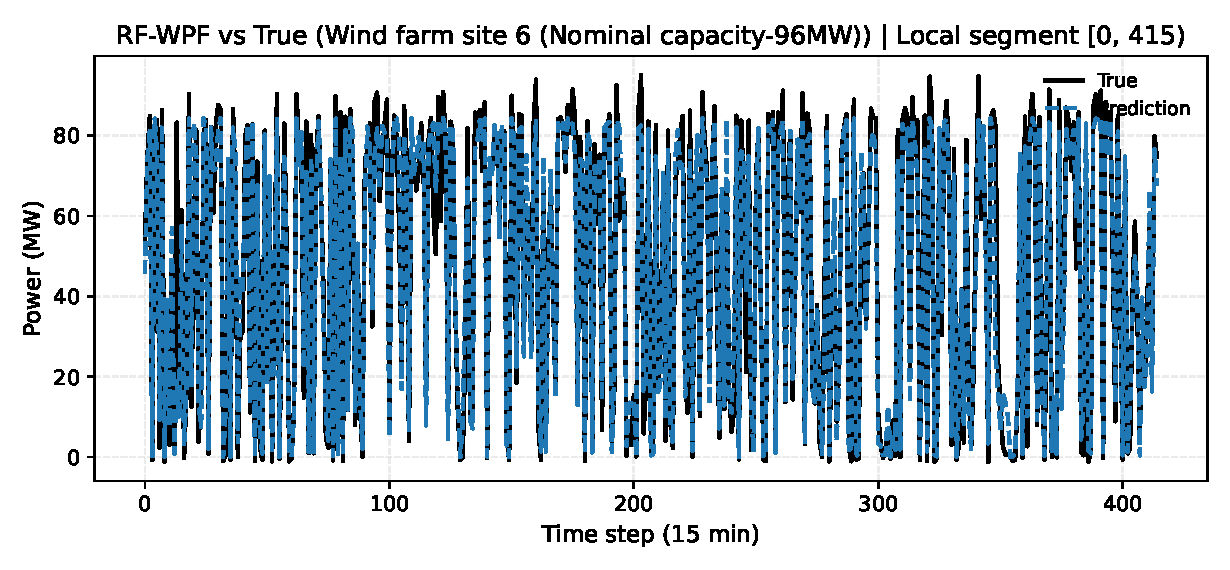
\includegraphics[width=0.96\linewidth]{experiment2/plots_selected/farm3_RF-WPF.pdf}
\end{minipage}\hfill
\begin{minipage}[t]{0.47\linewidth}
\centering
(j) TL-QLDMR\par
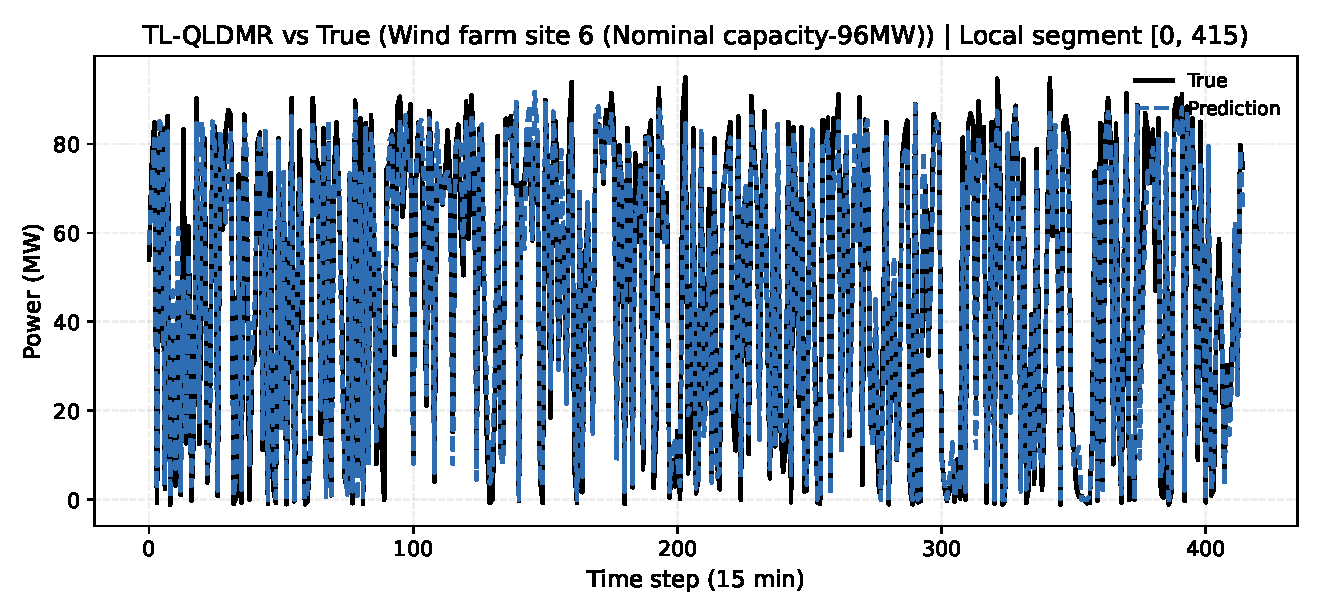
\includegraphics[width=0.96\linewidth]{experiment2/plots_selected/farm3_TL-QLDMR.pdf}
\end{minipage}
\caption{{\color{blue}Archived manuscript values (not recomputed): }Prediction comparison over selected temporal segments on the Farm~6 extreme-event test set (Part V).}
\label{fig:exp2_curves_e}
\end{figure}

{\color{blue}Table~\ref{tab:exp2_results} and Figs.~\ref{fig:exp2_curves_a}--\ref{fig:exp2_curves_e} retain the archived point-prediction scores and traces. The archived manuscript table gives RMSE 7.478 for the earlier TL-QLDMR implementation, 7.603 for HHO-SVR, and 7.967 for RF-WPF. These numerical differences do not validate the corrected residual-variance objective or establish the effect of variance symmetry. The primary chronological evaluation reports predictions generated by the centered-residual implementation under a common documented protocol.}


The earlier point-prediction experiment injected Gaussian noise into training and testing inputs at signal-to-noise ratios (SNRs) of 60, 40, and 30\,dB.
The $R^2$ results under different noise levels are summarized in Table~\ref{tab:exp2_noise}.

\begin{table}[ht]
\centering
\caption{{\color{blue}Archived manuscript values (not recomputed): }Model performance ($R^2$) under varying SNR on the Farm~6 extreme-event test set.}
\setlength{\tabcolsep}{3.5mm}
\begin{tabular}{lccc}
\toprule
Model & SNR = 30 dB & SNR = 40 dB & SNR = 60 dB \\
\midrule
LDMR & 0.9084 & 0.9080 & 0.9084 \\
BLSSVR        & 0.9121 & 0.9146 & 0.9154 \\
ARA-SVR       & 0.9311 & 0.9316 & 0.9316 \\
FLSVR         & 0.9380 & 0.9381 & 0.9381 \\
SVR  & 0.9409 & 0.9414 & 0.9413 \\
HHO-SVR       & 0.9442 & 0.9438 & 0.9437 \\
BRF-WPF       & 0.9177 & 0.9250 & 0.9253 \\
KMeans-GBT    & 0.9209 & 0.9230 & 0.9262 \\
RF-WPF        & 0.9471 & 0.9485 & 0.9469 \\
\textbf{TL-QLDMR (Ours)} & \textbf{0.9584} & \textbf{0.9560} & \textbf{0.9603} \\
\bottomrule
\end{tabular}
\label{tab:exp2_noise}
\end{table}

{\color{blue}Table~\ref{tab:exp2_noise} retains the archived noise-perturbation scores. They concern the earlier implementation and do not establish noise resilience of the corrected centered-residual model.}

{\color{blue}The earlier few-shot results are not used to assess the corrected model because their solver version has not been established. The chronological scarcity study in Section~\ref{sec:chronological} instead uses explicit target fitting counts, nested random subsets, a fixed test period, and a fixed total coefficient mass for each domain. All three predefined seeds are reported.}

%---------------- Experiment 3 --------------------%
\subsection{Earlier interval-prediction and noise experiments}\label{sec:exp3}

{\color{blue}The archived interval-prediction comparison reports a nominal coverage of 95\%. These retained scores describe earlier model and calibration runs; they are not evidence of coverage or sharpness for the corrected objective.}


The interval prediction baselines include SVQR, twin support vector quantile regression (TSVQR) \citep{tsvqr2023}, a robust truncated-pinball SVQR baseline (UQSVM-SSVQR) \citep{wang2024ssvqr}, nonlinear feature selection SVQR (NFS-SVQR) \citep{ye2025nfs}, $\nu$-support vector regression with conformalized intervals (NuSVR-CI) \citep{romano2019cqr}, robust low-rank multiple kernel learning (RLMKL) \citep{jiang2021rlmkl}, a hybrid deep-learning interval model (HybridDL-Interval) \citep{hybriddl2025}, an attention-based recurrent neural network interval model (AMQRNN) \citep{amqrnn2025}, quantile gradient boosted regression (QGBR) \citep{hu2025ncqgbr}, and conformalized quantile regression multilayer perceptron (CQR-MLP) \citep{hu2025nescqr}.

{\color{blue}Table~\ref{tab:exp3_results} retains historical interval scores at nominal 95\% prediction coverage ($\alpha=0.05$); it does not report confidence intervals for model parameters.}

\begin{table*}[ht]
\centering
\caption{{\color{blue}Archived manuscript values (not recomputed): }Interval prediction results on the extreme-event test set of Farm~6 at nominal 95\% prediction coverage ($\alpha = 0.05$).}
\setlength{\tabcolsep}{4mm}
\begin{tabular}{lccccc}
\toprule
Model & PICP & MPIW & PINAW & CWC & Winkler \\
\midrule
NuSVR-CI            & 0.843 & \textbf{19.970} & \textbf{0.208} & 0.285 & 54.603 \\
HybridDL-Interval   & 0.954 & 31.645 & 0.329 & 0.329 & 60.224 \\
RLMKL               & 0.957 & 31.804 & 0.331 & 0.331 & 39.275 \\
TSVQR               & 0.889 & 24.592 & 0.256 & 0.342 & 48.178 \\
SVQR       & \textbf{0.959} & 34.342 & 0.357 & 0.357 & 42.067 \\
QGBR                & 0.949 & 31.715 & 0.330 & 0.429 & 37.643 \\
CQR-MLP             & 0.942 & 31.750 & 0.330 & 0.431 & 46.772 \\
AMQRNN              & 0.940 & 32.432 & 0.337 & 0.441 & 66.874 \\
NFS-SVQR            & 0.913 & 68.359 & 0.711 & 0.941 & 76.997 \\
UQSVM-SSVQR         & 0.928 & 81.710 & 0.850 & 1.117 & 85.162 \\
\textbf{TL-QLDMR (Ours)} & \textbf{0.959} & 25.791 & 0.268 & \textbf{0.268} & \textbf{34.506} \\
\bottomrule
\end{tabular}
\label{tab:exp3_results}
\end{table*}

{\color{blue}The archived TL-QLDMR row has PICP 0.959 and CWC 0.268. Neither the numerical ordering of the retained rows nor the displayed forecast traces establishes a calibration advantage for the corrected model. The primary chronological interval evaluation instead uses disjoint fitting, calibration, and test labels.}


The earlier interval experiment injected Gaussian noise into test inputs at SNR $\in \{60,40,30\}$ dB.
Table~\ref{tab:exp3_noise} reports the full set of interval metrics under this noisy-test protocol.

\FloatBarrier

\begin{table*}[ht]
\centering
\caption{{\color{blue}Archived manuscript values (not recomputed): }Interval prediction results under varying SNR on the extreme-event test set of Farm~6 at nominal 95\% prediction coverage ($\alpha = 0.05$).}
\setlength{\tabcolsep}{3.0mm}
\begin{tabular}{llccccc}
\toprule
Model & SNR (dB) & PICP & MPIW & PINAW & CWC & Winkler \\
\midrule
\multirow{3}{*}{NuSVR-CI}
  & 30 & 0.8386 & \textbf{19.970} & \textbf{0.2077} & 0.2856 & 54.922 \\
  & 40 & 0.8361 & \textbf{19.970} & \textbf{0.2077} & 0.2860 & 54.623 \\
  & 60 & 0.8434 & \textbf{19.970} & \textbf{0.2077} & 0.2849 & 54.588 \\
\multirow{3}{*}{HybridDL-Interval}
  & 30 & 0.9422 & 32.304 & 0.3360 & 0.4384 & 53.462 \\
  & 40 & 0.9422 & 32.307 & 0.3361 & 0.4385 & 53.420 \\
  & 60 & 0.9422 & 32.306 & 0.3361 & 0.4385 & 53.408 \\
\multirow{3}{*}{RLMKL}
  & 30 & 0.9494 & 30.161 & 0.3138 & 0.4080 & 39.063 \\
  & 40 & 0.9494 & 30.101 & 0.3131 & 0.4072 & 39.235 \\
  & 60 & 0.9494 & 30.095 & 0.3131 & 0.4071 & 39.200 \\
\multirow{3}{*}{TSVQR}
  & 30 & 0.8892 & 24.570 & 0.2556 & 0.3422 & 48.306 \\
  & 40 & 0.8892 & 24.588 & 0.2558 & 0.3424 & 48.140 \\
  & 60 & 0.8892 & 24.592 & 0.2558 & 0.3425 & 48.169 \\
\multirow{3}{*}{SVQR}
  & 30 & 0.9446 & 29.704 & 0.3090 & 0.4027 & 41.541 \\
  & 40 & 0.9422 & 29.725 & 0.3092 & 0.4034 & 41.429 \\
  & 60 & 0.9446 & 29.728 & 0.3092 & 0.4030 & 41.420 \\
\multirow{3}{*}{QGBR}
  & 30 & 0.9518 & 32.067 & 0.3336 & 0.3336 & 38.441 \\
  & 40 & 0.9518 & 31.721 & 0.3300 & 0.3300 & 37.424 \\
  & 60 & 0.9470 & 31.706 & 0.3298 & 0.4294 & 37.750 \\
\multirow{3}{*}{CQR-MLP}
  & 30 & 0.9325 & 32.548 & 0.3386 & 0.4438 & 48.828 \\
  & 40 & 0.9325 & 32.550 & 0.3386 & 0.4438 & 48.780 \\
  & 60 & 0.9325 & 32.554 & 0.3386 & 0.4438 & 48.743 \\
\multirow{3}{*}{AMQRNN}
  & 30 & 0.9518 & 33.517 & 0.3487 & 0.3487 & 68.546 \\
  & 40 & 0.9518 & 33.513 & 0.3486 & 0.3486 & 68.517 \\
  & 60 & 0.9518 & 33.512 & 0.3486 & 0.3486 & 68.515 \\
\multirow{3}{*}{NFS-SVQR}
  & 30 & 0.9060 & 68.369 & 0.7112 & 0.9442 & 77.305 \\
  & 40 & 0.9133 & 68.376 & 0.7113 & 0.9409 & 76.878 \\
  & 60 & 0.9133 & 68.359 & 0.7111 & 0.9407 & 76.983 \\
\multirow{3}{*}{UQSVM-SSVQR}
  & 30 & 0.9229 & 81.706 & 0.8499 & 1.1191 & 85.364 \\
  & 40 & 0.9277 & 81.718 & 0.8501 & 1.1167 & 85.178 \\
  & 60 & 0.9277 & 81.710 & 0.8500 & 1.1166 & 85.162 \\
\multirow{3}{*}{\textbf{TL-QLDMR (Ours)}}
  & 30 & \textbf{0.9542} & 26.709 & 0.2778 & \textbf{0.2778} & \textbf{36.307} \\
  & 40 & \textbf{0.9566} & 26.713 & 0.2779 & \textbf{0.2779} & \textbf{36.034} \\
  & 60 & \textbf{0.9566} & 26.715 & 0.2779 & \textbf{0.2779} & \textbf{36.083} \\
\bottomrule
\end{tabular}
\label{tab:exp3_noise}
\end{table*}

{\color{blue}The retained noisy-input interval scores belong to the earlier implementation. A robustness conclusion for the corrected model requires repeating the perturbation protocol without using test outcomes to tune interval widths or coverage.}



%---------------- Experiment 4 --------------------%
\subsection{Centered-residual evaluation on the historical random split}\label{sec:exp4}

{\color{blue}Implementation checks address the mathematical consistency of the corrected centered-residual objective. Small deterministic tests compare the direct centered-residual penalty with its quadratic expansion, check analytical gradients by finite differences, verify mini-batch scaling, and compare the exact-kernel solution with an independently constructed primal QP. Distinct and repeated inputs are included to exercise both positive-definite and singular Gram matrices. These checks pass; they establish implementation consistency on the tested cases, not forecasting performance or a general optimization-rate theorem.}

{\color{blue}The empirical ablation protocol comprises four models: the full corrected objective; the same model with $\lambda_1=0$; the same model with $\lambda_2=0$; and a target-only model using centered target residuals and no inter-domain penalty. A separate symmetric-versus-asymmetric residual-variance ablation is not defined, because the full model already uses a symmetric variance term.}


\begin{table*}[htbp]
\centering
{\color{blue}
\caption{\textcolor{blue}{Fixed-configuration results of the corrected objective on the same 415 Farm~6 test windows. All four variants are reported. Point and interval tasks use their respective configurations in Section~\ref{app:legacy_setup}; interval endpoints use training-pool calibration only. These are single-seed historical-split diagnostics on the supplied processed data.}}
\label{tab:corrected_diagnostic}
\setlength{\tabcolsep}{3pt}
\begin{tabular}{lrrr}
\toprule
Model & RMSE (MW) & MAE (MW) & $R^2$ \\
\midrule
Full & 7.531988 & 5.324838 & 0.954594 \\
No variance & 7.531987 & 5.324836 & 0.954594 \\
No projected discrepancy & 7.636272 & 5.345320 & 0.953328 \\
Target only & 8.120599 & 5.144528 & 0.947220 \\
\bottomrule
\end{tabular}

\vspace{2mm}
\begin{tabular}{lrrrrr}
\toprule
Model & PICP & MPIW (MW) & PINAW & CWC & Winkler (MW) \\
\midrule
Full & 0.971084 & 27.698317 & 0.288131 & 0.288131 & 34.935618 \\
No variance & 0.971084 & 27.698314 & 0.288131 & 0.288131 & 34.935616 \\
No projected discrepancy & 0.971084 & 28.194452 & 0.293292 & 0.293292 & 35.739322 \\
Target only & 0.978313 & 31.882089 & 0.331653 & 0.331653 & 37.223778 \\
\bottomrule
\end{tabular}
}
\end{table*}

{\color{blue}Table~\ref{tab:corrected_diagnostic} reports the complete fixed-configuration comparison, including results that do not support a component benefit. The full and no-variance fits differ in point-prediction RMSE by less than $10^{-6}$ MW, so this setting does not demonstrate a predictive benefit from the variance term. The target-only model has higher RMSE but lower MAE than the full model; there is no uniform ranking across these point metrics. The calibrated interval results describe empirical coverage and width on this split, not a general coverage guarantee. A single seed and one inherited configuration do not establish statistical significance or the optimality of the regularization weights.}

{\color{blue}The earlier SymVar component scores and residual-density figure remain excluded: the full corrected model already has a symmetric variance term, the archived SymVar point metrics are inconsistent with a common test-label variance, and some archived interval scores used test-dependent post-processing. The new results are generated separately, with saved models, predictions, split identifiers, and calibration scores. They do not rehabilitate the earlier component comparison. The separate chronological evaluation in Section~\ref{sec:chronological} supplies a documented cleaning and time-split protocol.}

\FloatBarrier


%---------------- Experiment 5 --------------------%
\subsection{Earlier solver timing records}\label{sec:exp5}

{\color{blue}The timing table retains measurements from the earlier CVXOPT, Torch-GD, batch-SGD, and Nystr\"{o}m implementations. The earlier batch-SGD and fast implementations did not optimize the same corrected residual-variance objective, so these measurements are not treated as an equal-objective solver comparison.}


The earlier timing experiment considered seven training scales, increasing the combined training size from 100 to the full $N=69{,}737$. The evaluated sizes are $N=100, 500, 1{,}000, 3{,}000, 10{,}000, 30{,}000$, and $69{,}737$.
For each configuration, wall-clock training time (seconds) is recorded. Table~\ref{tab:scalability_results} summarizes the results.

\begin{table}[ht]
\centering
\caption{{\color{blue}Archived manuscript values (not recomputed): }Training time (seconds) of four solvers over expanding training scales on Farm~6. ``---'' denotes runs not extended further because of prohibitive computational cost.}
{\small
\setlength{\tabcolsep}{2.6mm}
\begin{tabular}{rcccc}
\toprule
$N$ & CVXOPT & Torch-GD & Batch SGD & Nystr\"{o}m-SGD (Ours) \\
\midrule
100      & 0.509 & 2.155 & 2.746 & \textbf{0.035} \\
500      & 1.052 & 2.618 & 4.637 & \textbf{1.035} \\
1{,}000  & 7.655 & 2.979 & 5.699 & \textbf{1.038} \\
3{,}000  & --- & 20.395 & 6.418 & \textbf{2.468} \\
10{,}000 & --- & --- & 10.401 & \textbf{2.703} \\
30{,}000 & --- & --- & 25.338 & \textbf{3.483} \\
69{,}737 & --- & --- & --- & \textbf{5.021} \\
\bottomrule
\end{tabular}
}
\label{tab:scalability_results}
\end{table}

{\color{blue}The table records the observed runtimes and stopping points of those implementations. Because their optimized objectives differ, the numerical ordering is not used to compare solver efficiency for the common objective in Section~\ref{novel}.}

{\color{blue}The recorded 5.021-second full-sample runtime belongs to the earlier fast implementation and is not assigned to the corrected solver. A valid accuracy--runtime comparison must use the same normalized objective, report optimization residuals or objective gaps, and include feature construction and regularizer multiplication costs. The dense-operation analysis in Section~\ref{fast_alg} specifies these costs without interpreting the archived timing table as validation. The new fixed-feature accuracy--runtime curves in Section~\ref{sec:chronological} measure the corrected solver across landmark and source-data sizes; they do not supply exact-QP objective gaps or certified approximation errors.}



